% Generated by Sphinx.
\def\sphinxdocclass{report}
\documentclass[a4paper,10pt,english]{sphinxmanual}
\usepackage[utf8]{inputenc}
\DeclareUnicodeCharacter{00A0}{\nobreakspace}
\usepackage{cmap}
\usepackage[T1]{fontenc}
\usepackage{babel}
\usepackage{times}
\usepackage[Bjarne]{fncychap}
\usepackage{longtable}
\usepackage{sphinx}
\usepackage{multirow}


\title{gWTO2 Documentation (Draft)}
\date{September 29, 2014}
\release{2.0RC}
\author{itoledo@alma.cl}
\newcommand{\sphinxlogo}{}
\renewcommand{\releasename}{Release}
\makeindex

\makeatletter
\def\PYG@reset{\let\PYG@it=\relax \let\PYG@bf=\relax%
    \let\PYG@ul=\relax \let\PYG@tc=\relax%
    \let\PYG@bc=\relax \let\PYG@ff=\relax}
\def\PYG@tok#1{\csname PYG@tok@#1\endcsname}
\def\PYG@toks#1+{\ifx\relax#1\empty\else%
    \PYG@tok{#1}\expandafter\PYG@toks\fi}
\def\PYG@do#1{\PYG@bc{\PYG@tc{\PYG@ul{%
    \PYG@it{\PYG@bf{\PYG@ff{#1}}}}}}}
\def\PYG#1#2{\PYG@reset\PYG@toks#1+\relax+\PYG@do{#2}}

\expandafter\def\csname PYG@tok@gd\endcsname{\def\PYG@tc##1{\textcolor[rgb]{0.63,0.00,0.00}{##1}}}
\expandafter\def\csname PYG@tok@gu\endcsname{\let\PYG@bf=\textbf\def\PYG@tc##1{\textcolor[rgb]{0.50,0.00,0.50}{##1}}}
\expandafter\def\csname PYG@tok@gt\endcsname{\def\PYG@tc##1{\textcolor[rgb]{0.00,0.27,0.87}{##1}}}
\expandafter\def\csname PYG@tok@gs\endcsname{\let\PYG@bf=\textbf}
\expandafter\def\csname PYG@tok@gr\endcsname{\def\PYG@tc##1{\textcolor[rgb]{1.00,0.00,0.00}{##1}}}
\expandafter\def\csname PYG@tok@cm\endcsname{\let\PYG@it=\textit\def\PYG@tc##1{\textcolor[rgb]{0.25,0.50,0.56}{##1}}}
\expandafter\def\csname PYG@tok@vg\endcsname{\def\PYG@tc##1{\textcolor[rgb]{0.73,0.38,0.84}{##1}}}
\expandafter\def\csname PYG@tok@m\endcsname{\def\PYG@tc##1{\textcolor[rgb]{0.13,0.50,0.31}{##1}}}
\expandafter\def\csname PYG@tok@mh\endcsname{\def\PYG@tc##1{\textcolor[rgb]{0.13,0.50,0.31}{##1}}}
\expandafter\def\csname PYG@tok@cs\endcsname{\def\PYG@tc##1{\textcolor[rgb]{0.25,0.50,0.56}{##1}}\def\PYG@bc##1{\setlength{\fboxsep}{0pt}\colorbox[rgb]{1.00,0.94,0.94}{\strut ##1}}}
\expandafter\def\csname PYG@tok@ge\endcsname{\let\PYG@it=\textit}
\expandafter\def\csname PYG@tok@vc\endcsname{\def\PYG@tc##1{\textcolor[rgb]{0.73,0.38,0.84}{##1}}}
\expandafter\def\csname PYG@tok@il\endcsname{\def\PYG@tc##1{\textcolor[rgb]{0.13,0.50,0.31}{##1}}}
\expandafter\def\csname PYG@tok@go\endcsname{\def\PYG@tc##1{\textcolor[rgb]{0.20,0.20,0.20}{##1}}}
\expandafter\def\csname PYG@tok@cp\endcsname{\def\PYG@tc##1{\textcolor[rgb]{0.00,0.44,0.13}{##1}}}
\expandafter\def\csname PYG@tok@gi\endcsname{\def\PYG@tc##1{\textcolor[rgb]{0.00,0.63,0.00}{##1}}}
\expandafter\def\csname PYG@tok@gh\endcsname{\let\PYG@bf=\textbf\def\PYG@tc##1{\textcolor[rgb]{0.00,0.00,0.50}{##1}}}
\expandafter\def\csname PYG@tok@ni\endcsname{\let\PYG@bf=\textbf\def\PYG@tc##1{\textcolor[rgb]{0.84,0.33,0.22}{##1}}}
\expandafter\def\csname PYG@tok@nl\endcsname{\let\PYG@bf=\textbf\def\PYG@tc##1{\textcolor[rgb]{0.00,0.13,0.44}{##1}}}
\expandafter\def\csname PYG@tok@nn\endcsname{\let\PYG@bf=\textbf\def\PYG@tc##1{\textcolor[rgb]{0.05,0.52,0.71}{##1}}}
\expandafter\def\csname PYG@tok@no\endcsname{\def\PYG@tc##1{\textcolor[rgb]{0.38,0.68,0.84}{##1}}}
\expandafter\def\csname PYG@tok@na\endcsname{\def\PYG@tc##1{\textcolor[rgb]{0.25,0.44,0.63}{##1}}}
\expandafter\def\csname PYG@tok@nb\endcsname{\def\PYG@tc##1{\textcolor[rgb]{0.00,0.44,0.13}{##1}}}
\expandafter\def\csname PYG@tok@nc\endcsname{\let\PYG@bf=\textbf\def\PYG@tc##1{\textcolor[rgb]{0.05,0.52,0.71}{##1}}}
\expandafter\def\csname PYG@tok@nd\endcsname{\let\PYG@bf=\textbf\def\PYG@tc##1{\textcolor[rgb]{0.33,0.33,0.33}{##1}}}
\expandafter\def\csname PYG@tok@ne\endcsname{\def\PYG@tc##1{\textcolor[rgb]{0.00,0.44,0.13}{##1}}}
\expandafter\def\csname PYG@tok@nf\endcsname{\def\PYG@tc##1{\textcolor[rgb]{0.02,0.16,0.49}{##1}}}
\expandafter\def\csname PYG@tok@si\endcsname{\let\PYG@it=\textit\def\PYG@tc##1{\textcolor[rgb]{0.44,0.63,0.82}{##1}}}
\expandafter\def\csname PYG@tok@s2\endcsname{\def\PYG@tc##1{\textcolor[rgb]{0.25,0.44,0.63}{##1}}}
\expandafter\def\csname PYG@tok@vi\endcsname{\def\PYG@tc##1{\textcolor[rgb]{0.73,0.38,0.84}{##1}}}
\expandafter\def\csname PYG@tok@nt\endcsname{\let\PYG@bf=\textbf\def\PYG@tc##1{\textcolor[rgb]{0.02,0.16,0.45}{##1}}}
\expandafter\def\csname PYG@tok@nv\endcsname{\def\PYG@tc##1{\textcolor[rgb]{0.73,0.38,0.84}{##1}}}
\expandafter\def\csname PYG@tok@s1\endcsname{\def\PYG@tc##1{\textcolor[rgb]{0.25,0.44,0.63}{##1}}}
\expandafter\def\csname PYG@tok@gp\endcsname{\let\PYG@bf=\textbf\def\PYG@tc##1{\textcolor[rgb]{0.78,0.36,0.04}{##1}}}
\expandafter\def\csname PYG@tok@sh\endcsname{\def\PYG@tc##1{\textcolor[rgb]{0.25,0.44,0.63}{##1}}}
\expandafter\def\csname PYG@tok@ow\endcsname{\let\PYG@bf=\textbf\def\PYG@tc##1{\textcolor[rgb]{0.00,0.44,0.13}{##1}}}
\expandafter\def\csname PYG@tok@sx\endcsname{\def\PYG@tc##1{\textcolor[rgb]{0.78,0.36,0.04}{##1}}}
\expandafter\def\csname PYG@tok@bp\endcsname{\def\PYG@tc##1{\textcolor[rgb]{0.00,0.44,0.13}{##1}}}
\expandafter\def\csname PYG@tok@c1\endcsname{\let\PYG@it=\textit\def\PYG@tc##1{\textcolor[rgb]{0.25,0.50,0.56}{##1}}}
\expandafter\def\csname PYG@tok@kc\endcsname{\let\PYG@bf=\textbf\def\PYG@tc##1{\textcolor[rgb]{0.00,0.44,0.13}{##1}}}
\expandafter\def\csname PYG@tok@c\endcsname{\let\PYG@it=\textit\def\PYG@tc##1{\textcolor[rgb]{0.25,0.50,0.56}{##1}}}
\expandafter\def\csname PYG@tok@mf\endcsname{\def\PYG@tc##1{\textcolor[rgb]{0.13,0.50,0.31}{##1}}}
\expandafter\def\csname PYG@tok@err\endcsname{\def\PYG@bc##1{\setlength{\fboxsep}{0pt}\fcolorbox[rgb]{1.00,0.00,0.00}{1,1,1}{\strut ##1}}}
\expandafter\def\csname PYG@tok@kd\endcsname{\let\PYG@bf=\textbf\def\PYG@tc##1{\textcolor[rgb]{0.00,0.44,0.13}{##1}}}
\expandafter\def\csname PYG@tok@ss\endcsname{\def\PYG@tc##1{\textcolor[rgb]{0.32,0.47,0.09}{##1}}}
\expandafter\def\csname PYG@tok@sr\endcsname{\def\PYG@tc##1{\textcolor[rgb]{0.14,0.33,0.53}{##1}}}
\expandafter\def\csname PYG@tok@mo\endcsname{\def\PYG@tc##1{\textcolor[rgb]{0.13,0.50,0.31}{##1}}}
\expandafter\def\csname PYG@tok@mi\endcsname{\def\PYG@tc##1{\textcolor[rgb]{0.13,0.50,0.31}{##1}}}
\expandafter\def\csname PYG@tok@kn\endcsname{\let\PYG@bf=\textbf\def\PYG@tc##1{\textcolor[rgb]{0.00,0.44,0.13}{##1}}}
\expandafter\def\csname PYG@tok@o\endcsname{\def\PYG@tc##1{\textcolor[rgb]{0.40,0.40,0.40}{##1}}}
\expandafter\def\csname PYG@tok@kr\endcsname{\let\PYG@bf=\textbf\def\PYG@tc##1{\textcolor[rgb]{0.00,0.44,0.13}{##1}}}
\expandafter\def\csname PYG@tok@s\endcsname{\def\PYG@tc##1{\textcolor[rgb]{0.25,0.44,0.63}{##1}}}
\expandafter\def\csname PYG@tok@kp\endcsname{\def\PYG@tc##1{\textcolor[rgb]{0.00,0.44,0.13}{##1}}}
\expandafter\def\csname PYG@tok@w\endcsname{\def\PYG@tc##1{\textcolor[rgb]{0.73,0.73,0.73}{##1}}}
\expandafter\def\csname PYG@tok@kt\endcsname{\def\PYG@tc##1{\textcolor[rgb]{0.56,0.13,0.00}{##1}}}
\expandafter\def\csname PYG@tok@sc\endcsname{\def\PYG@tc##1{\textcolor[rgb]{0.25,0.44,0.63}{##1}}}
\expandafter\def\csname PYG@tok@sb\endcsname{\def\PYG@tc##1{\textcolor[rgb]{0.25,0.44,0.63}{##1}}}
\expandafter\def\csname PYG@tok@k\endcsname{\let\PYG@bf=\textbf\def\PYG@tc##1{\textcolor[rgb]{0.00,0.44,0.13}{##1}}}
\expandafter\def\csname PYG@tok@se\endcsname{\let\PYG@bf=\textbf\def\PYG@tc##1{\textcolor[rgb]{0.25,0.44,0.63}{##1}}}
\expandafter\def\csname PYG@tok@sd\endcsname{\let\PYG@it=\textit\def\PYG@tc##1{\textcolor[rgb]{0.25,0.44,0.63}{##1}}}

\def\PYGZbs{\char`\\}
\def\PYGZus{\char`\_}
\def\PYGZob{\char`\{}
\def\PYGZcb{\char`\}}
\def\PYGZca{\char`\^}
\def\PYGZam{\char`\&}
\def\PYGZlt{\char`\<}
\def\PYGZgt{\char`\>}
\def\PYGZsh{\char`\#}
\def\PYGZpc{\char`\%}
\def\PYGZdl{\char`\$}
\def\PYGZhy{\char`\-}
\def\PYGZsq{\char`\'}
\def\PYGZdq{\char`\"}
\def\PYGZti{\char`\~}
% for compatibility with earlier versions
\def\PYGZat{@}
\def\PYGZlb{[}
\def\PYGZrb{]}
\makeatother

\renewcommand\PYGZsq{\textquotesingle}

\begin{document}

\maketitle
\tableofcontents
\phantomsection\label{index::doc}


\code{Download documentation in PDF}.


\chapter{Introduction}
\label{intro2:introduction}\label{intro2:gwto2-documentation-contents}\label{intro2::doc}\begin{figure}[htbp]
\centering
\capstart

\scalebox{0.600000}{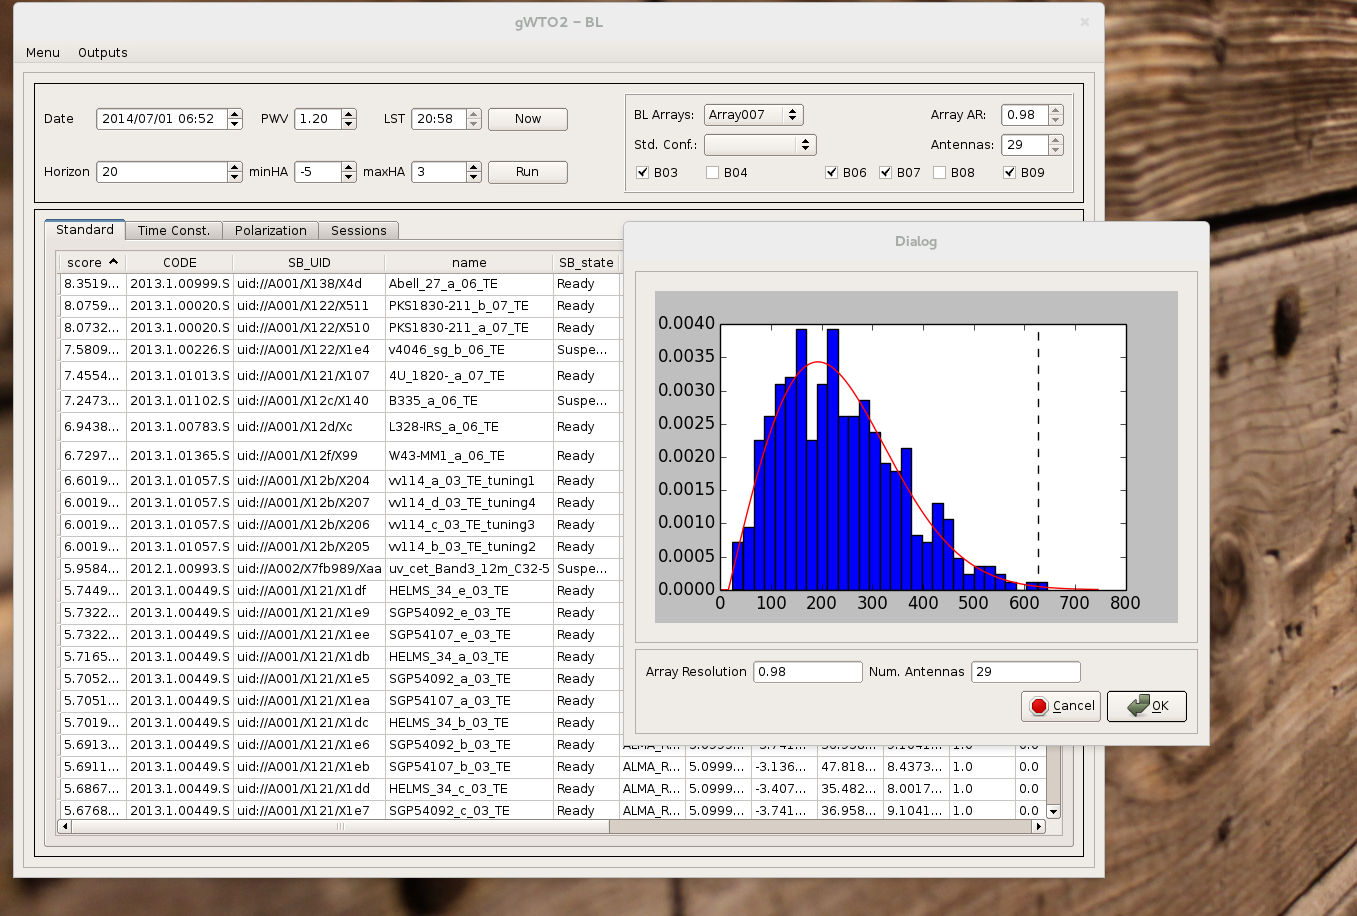
\includegraphics{Selection_003.png}}
\caption{Screenshot of gWTO2 RC}\end{figure}


\section{Goal}
\label{intro2:goal}
gWTO2 (gui for What To Observe cycle 2) is a real-time scheduler that uses both
a selection and score algorithms to select the best SB to observe given the
current conditions. However, its main goal is to provide a flexible and dynamic
benchmark where to test and optimize the algorithms that are being use in the
official scheduling tool for ALMA: the Dynamical Schedulling Algorithm (DSA).

The criteria behind gWTO2 comes from \href{http://almascience.eso.org/documents-and-tools/cycle-2/alma-proposers-guide}{Alma Cycle 2 Proposer Guide} (http://almascience.eso.org/documents-and-tools/cycle-2/alma-proposers-guide):
\begin{quote}

Science observations will be executed by ALMA operations staff, taking into
account (in rough order of priority): the weather conditions,
the configuration of the array, target elevation and other practical
constraints, the projects’ assigned priority group, and executive balance.
All other things being equal, the project with the highest scientific rank
will be observed.''

\begin{flushright}
---\emph{Section 5.1 of the ALMA Cycle 2 Proposers Guide.}
\end{flushright}
\end{quote}


\section{Considerations and problem description}
\label{intro2:considerations-and-problem-description}
It is easy at any given time to use these criteria to create an algorithm that
selects the best SB to run, given the current pwv, array configuration,
number of antennas and the target's horizontal coordinates; however the
algorithm needs to be more complex to achieve an optimal efficiency in the use
of telescope time. This optimal efficiency is defined as obtaining the maximum
scientific output given the avilable observing time.


\chapter{Using gWTO2}
\label{usingwto:using-gwto2}\label{usingwto::doc}

\section{Starting the GUI}
\label{usingwto:starting-the-gui}
gWTO2 is tested and deployed at the \textbf{osf-red} machine, within the \textbf{aod} account.
A virtual environment of python, based on the
\href{http://docs.continuum.io/anaconda/index.html}{Anaconda distribution} (http://docs.continuum.io/anaconda/index.html),
must be loaded before using it. This is achieved by running:

\begin{Verbatim}[commandchars=\\\{\}]
. activateC2Test
\end{Verbatim}

The Anaconda distribution is based on python 2.7.6 and includes numpy, pandas,
pyephem and other libraries need by gWTO.

The gui is run executing the gWTO2.py comand:

\begin{Verbatim}[commandchars=\\\{\}]
Usage: gWTO2.py arg1 [options]
    arg1 must be BL or ACA

Options:
  \PYGZhy{}h, \PYGZhy{}\PYGZhy{}help            show this help message and exit
  \PYGZhy{}c, \PYGZhy{}\PYGZhy{}clean           Force clean up of gWTO2 cache
  \PYGZhy{}p PATH, \PYGZhy{}\PYGZhy{}path=PATH  Path for cache
\end{Verbatim}

So, to run gWTO2 for baseline correlator use argument \emph{\texttt{BL}}, and
\emph{\texttt{ACA}} for Total Power and ACA. The \emph{\texttt{-c}} option should only be
used once per day.

I would also recommend to set the option \emph{\texttt{-p}} to something like
\code{'/.wto\_myname/'} so different users running gWTO won't mess up the cache
for each other. \textbf{After playing with gWTO2 using a different path, please}
\textbf{delete the directory created with the name .wto\_myname}


\section{The gWTO2 window}
\label{usingwto:the-gwto2-window}
After starting \textbf{gWTO2 BL} you will be presented with the gui shown on
{\hyperref[usingwto:fig2]{\emph{Figure 2}}} (\autopageref*{usingwto:fig2}).
If the \emph{\texttt{-c}} option was used, or the cache have been manually erased it,
the time until the gui is ready can be up to 5-7 minutes.
\begin{figure}[htbp]
\centering
\capstart

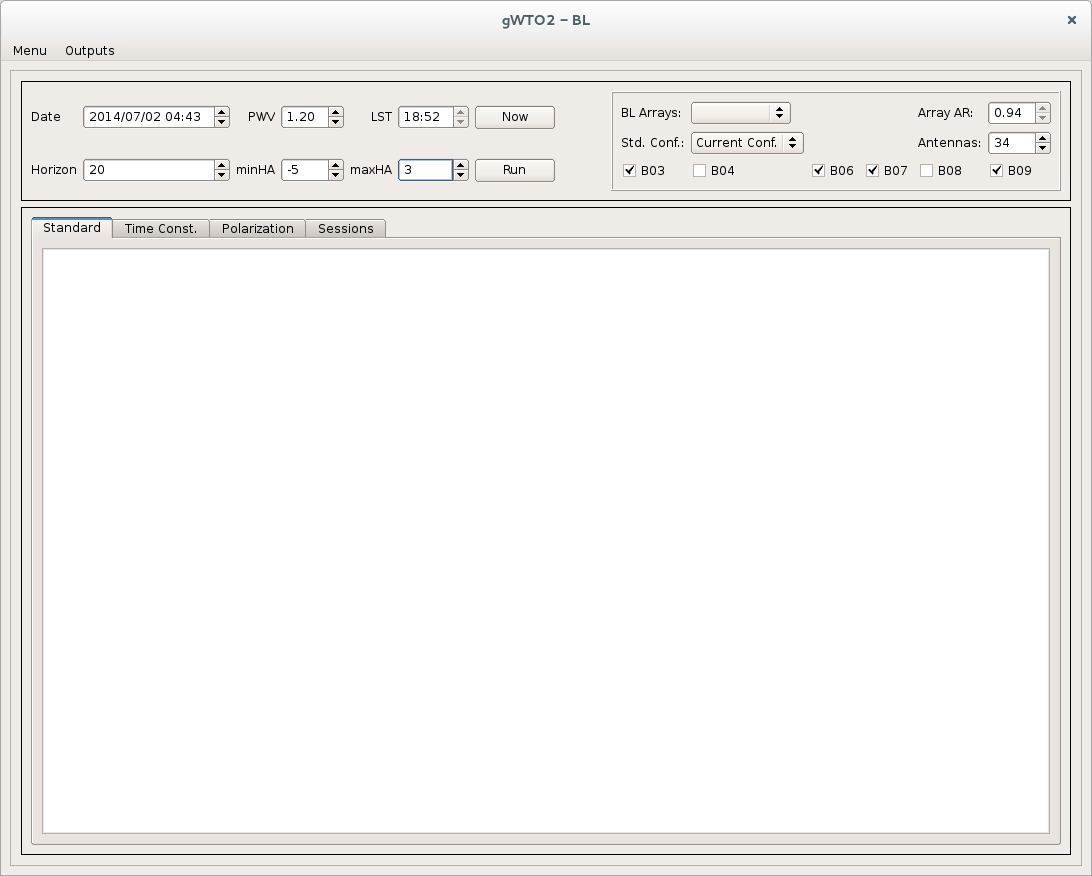
\includegraphics{gWTO2__BL_001.png}
\caption{Figure 2}\label{usingwto:fig2}\end{figure}

The gui for ACA (\textbf{gWTO2 ACA}) is almost the same, except for the lack
of \emph{Array Options}, and the presence of a tab \emph{TP} that
will be used for handling Total Power SBs.


\section{Setting up variables}
\label{usingwto:setting-up-variables}
After opening, the \emph{Date} will be by default the current UTC time,
\emph{PWV} is set to 1.2 mm., the \emph{Horizon} limit is 20 degrees,
\emph{minHA}, minimum hour angle, is -5 and \emph{maxHA}, maximum
hour angle, is 3. The \emph{LST} field is not editable, and it shows the
LST for the date/time set in the \emph{Date} field.
\begin{description}
\item[{\textbf{(For BL GUI only.)}}] \leavevmode
The box with the array variables will have the
\emph{Std. Conf.:} field set to \code{Current Conf.}
This \code{Current Conf.} comes from the output of the CASA script
\textbf{arrayConfigurationTools.py}, which can be found at
\code{\textasciitilde{}/AIV/science/ArrayConfiguration/Tools/arrayConfigurationTools.py}.
It is made with the antennas that in principle can be used for the current
ES Block. \textbf{It is the AoD Lead's duty to create the relevant files from}
\textbf{time to time to account for antenna movements or new antennas added}.
{\hyperref[apendix:current-conf]{\emph{(Instructions)}}} (\autopageref*{apendix:current-conf})

\item[{\textbf{(For BL GUI only.)}}] \leavevmode
The values given at \emph{Array AR:}  and \emph{Antennas:}
are set according to the \emph{current array's} angular resolution and
number of antennas offered officially for cycle 2.
\textbf{The only field you can modify at this stage in the `Antenna'}
\textbf{field, which is the number of antennas}. The idea is that the user will use
this information to have an idea of the current configuration characteristics,
and to run gWTO2 to plan observations ahead of time, or when Baseline arrays
have not been created in the last 6 to 12 hours.

\item[{\textbf{(For BL GUI only, when observing.)}}] \leavevmode
The user should press the button \emph{Now}, and a pop up window
similar to the one shown in {\hyperref[usingwto:fig3]{\emph{Figure 3}}} (\autopageref*{usingwto:fig3}) will appear.

\end{description}
\begin{figure}[htbp]
\centering
\capstart

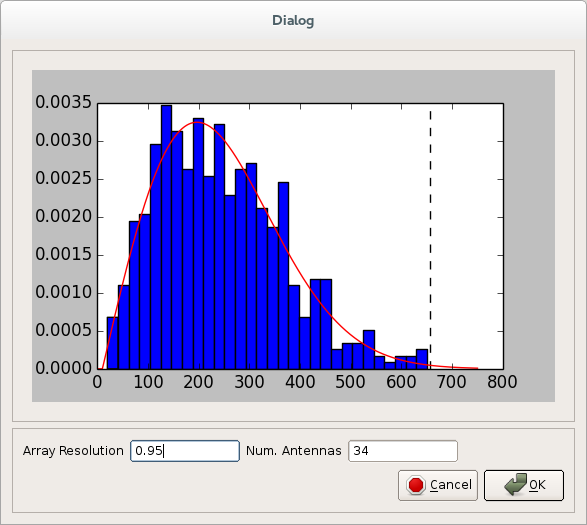
\includegraphics{gWTO2__BL_002.png}
\caption{Figure 3}\label{usingwto:fig3}\end{figure}

The window show the normalized histogram of the baseline lengths, and a fit to
this distribution, taking the data from latest Baseline Array created.
From this distribution the array's resolution is estimated, and the number of
antennas is also show. \textbf{The user should check that the array resolution is}
\textbf{close the the ``Current Conf.'' value, and that no outliers are fitted}. If
happy press the \emph{OK} button, and this will set the
\emph{Array AR:} and \emph{Antennas:} fields
in the main window. If \emph{Cancel} is pressed instead, the main window
will go back to \code{Current Conf.}. Also, when accepting the new array
estimates you will not longer be able to change the number of antennas unless
you go back to :keyword''\emph{Current Conf.}

The \emph{BL Arrays:} Combo menu is also populated with the list of the
baselines arrays created in the last 6 to 12 hours.
\begin{description}
\item[{\textbf{For ACA GUI only}}] \leavevmode
The number of antennas is 9 by default. Change the number according to the
number of antennas that are available.

\end{description}


\section{Running}
\label{usingwto:running}
When you are happy with the \emph{Date}, \emph{PWV} and
array variables (also the \emph{Horizon}, \emph{minHA} and
\emph{maxHA} values) you can run the selector and scoring algorithms
pressing the button \emph{Run}.

After an interval of a few seconds (5 to 15 seconds) you will be presented
with something similar to {\hyperref[usingwto:fig4]{\emph{Figure 4}}} (\autopageref*{usingwto:fig4}).
\begin{figure}[htbp]
\centering
\capstart

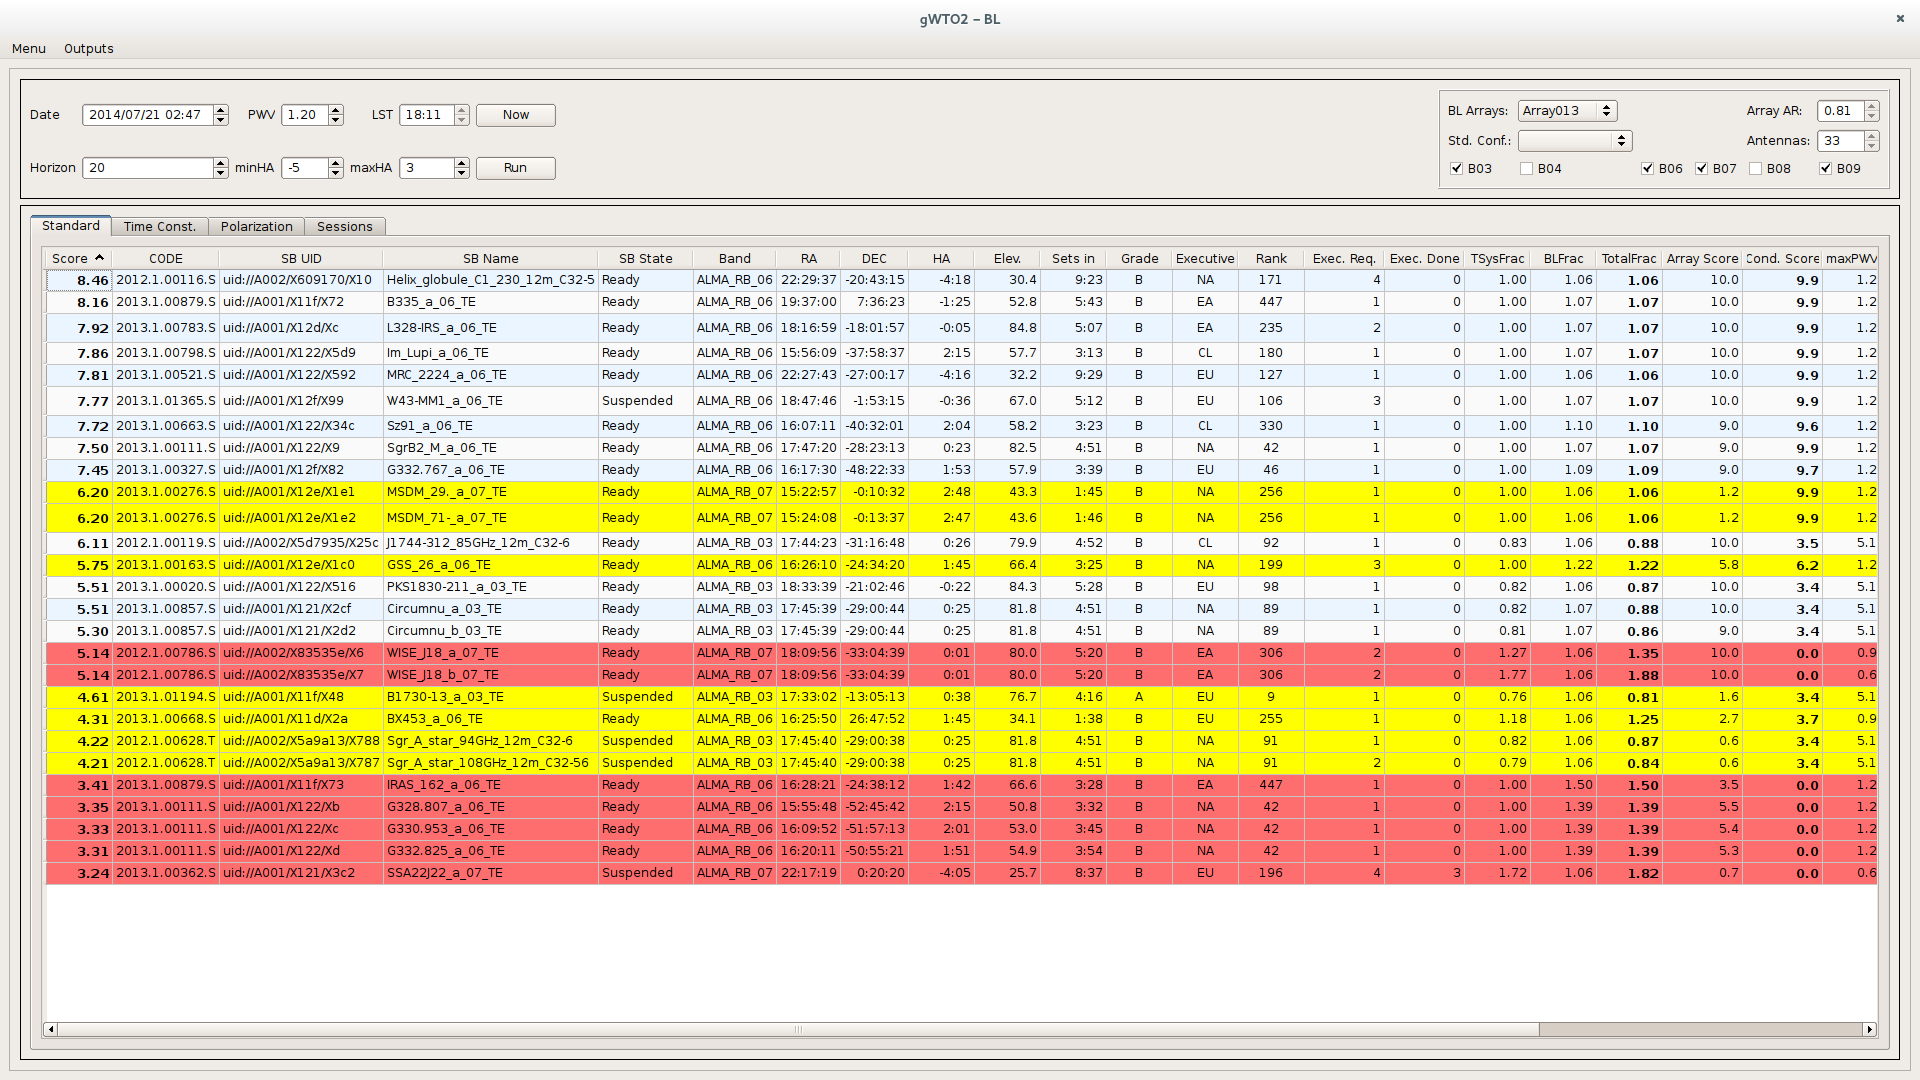
\includegraphics{gWTO2__BL_003.png}
\caption{Figure 4}\label{usingwto:fig4}\end{figure}


\section{Reading the output Scores}
\label{usingwto:reading-the-output-scores}

\subsection{Meaning of the background colors}
\label{usingwto:meaning-of-the-background-colors}\begin{itemize}
\item {} 
\textbf{Red}: Means that the integration time for the science target needs to be
increased by over a factor of 1.3 to reach the PI requested sensitivity.
\textbf{Do not change the integration time unless a clear policy has been set.}
\textbf{(AoD leader should know.)}

\item {} 
\textbf{Yellow}: The SB, even when it can be run with the current Array's angular
resolution, does require, or prefers, another configuration. If there is
nothing else to observe, the AoD could execute it. \textbf{This doesn't apply to}
\textbf{point sources.}

\end{itemize}


\subsection{Standard (ACA) Tab in BL (ACA) GUI}
\label{usingwto:standard-aca-tab-in-bl-aca-gui}\begin{enumerate}
\item {} 
\textbf{Score:} The score is the weighted mean of different scores calculated
for each observable SB. The score is a value between 0 and 10,
10 being the highest score.
\begin{enumerate}
\item {} 
Condition Score, 35\%. A score depending on the current PWV, number of
available antennas, and pwv used by the OT.

\item {} 
Array Score, 20\%. Depends in how close to the current array's resolution
is the SB asked angular resolution. For ACA and TP this is fixed to 10.

\item {} 
SB Completition Score, 15\%. SBs already started and closer to be completed
get higher scores

\item {} 
Letter Grade Score, 15\%. Score given by Cycle and letter grade.

\item {} 
Executive Score, 10\%. Score given by the executive of the Project.

\item {} 
Science Rank Score, 5\%. Score given by the scientific ranking of the
project.

\end{enumerate}

\item {} 
\textbf{CODE:} Project Code

\item {} 
\textbf{SB UID:} Scheduling Block's UID

\item {} 
\textbf{SB Name:} Scheduling Block's Name

\item {} 
\textbf{SB State:} Scheduling Block's state, or status, taken from the project
tracker

\item {} 
\textbf{Band:} Receiver(s) asked by the SB.

\item {} 
\textbf{RA:} Representative Right Ascension.

\item {} 
\textbf{DEC:} Representative Declination.

\item {} 
\textbf{HA:} Hour Angle for the given date and time.

\item {} 
\textbf{Elev.:} Elevation, in degrees, for the given date and time.

\item {} 
\textbf{Sets in:} Time left until the first of the field sources (science targets)
goes down the horizon limit. \emph{This calculated by checking the field sources}
\emph{coordinates of the SB, and not by the representative coordinates.}

\item {} 
\textbf{Grade:} Grade letter for the SB's project.

\item {} 
\textbf{Executive:} SB's project executive.

\item {} 
\textbf{Rank:} SB's Project science rank

\item {} 
\textbf{Exec. Req.:} Number of executions requested for this SB.

\item {} 
\textbf{Exec. Done.:} Number of execution blocks for this SB, that have the QA0
status set to PASS, or in Unset state.

\item {} 
\textbf{TsysFrac:} Given the TSys assumed by the PI in the OT, and the actual TSys
with the given pwv, this is the multiplicative factor for the time on source
(integration time) to reach the sensitivity asked by the PI. E.G., if the
TSysFrac is 0.8 it means that with the 80\% of the asked integration time the
rms will be achieved.

\item {} 
\textbf{BLFrac.:} Given the current number of antennas and array configuration the
number of usable baselines is calculated, and is compared with the SB
requirements, e.g., 34 antennas for BL, 9 for ACA. The ratio of these two
number gives the corrective factor needed to achieve the PI requested rms.
E.G., if the factor is 1.22, it means that the ToS should be a 22\% higher to
achieve the rms.

\item {} 
\textbf{TotalFrac.:} The total multiplicative factor for the time on source needed
given the calculated TsysFrac and BLFrac. If TotalFrac is higher than 1.3,
which means that if the SB is run with these conditions the rms achieved
would be sqrt(1/1.3) \textasciitilde{} 87\% of the asked rms, the whole row will have a
red background.
\textbf{This does not mean the AoD should change the ToS, unless}
\textbf{a clear policy has been given by PMG or the ES leader.}

\item {} 
\textbf{Array Score:} The array score, given for information purposes.

\item {} 
\textbf{Cond. Score:} The condition score, given for information purposes.

\item {} 
\textbf{maxPWVC:} The PWV used by the PI/P2G on the OT to calculate how much
integration time is needed to get the sensitivy requested.

\item {} 
\textbf{ArrayMinAR:} The minimum array's resolution that the current SB will
accept. This value comes from Stephane's script, and is corrected for all SBs
to the equivalent resolution at a 100GHZ and a source that would transit at
zenith.

\item {} 
\textbf{ArrCorr:} The angular resolution requiered by the SB, corrected to the
equivalent resolution at 100GHz and source with DEC -23.

\item {} 
\textbf{ArrayMinAR:} The maximum array's resolution that the current SB will
accept.

\item {} 
\textbf{Point Source:} are the targets of the SB point sources?

\item {} 
\textbf{TimeOnSource:} Integration time, in seconds, for the science target(s).
In the case of multisources, this time should be multiplied by the number of
sources.

\item {} 
\textbf{PRJ UID:} The SB's project UID.

\end{enumerate}


\chapter{Selection and Score algorithms}
\label{algorithm:selection-and-score-algorithms}\label{algorithm::doc}

\section{Selection and Data preparation}
\label{algorithm:selection}\label{algorithm:selection-and-data-preparation}
({\hyperref[wtoapi:wtoAlgorithm.WtoAlgorithm.selector]{\code{wtoAlgorithm.WtoAlgorithm.selector()}}} (\autopageref*{wtoapi:wtoAlgorithm.WtoAlgorithm.selector}))
\begin{enumerate}
\item {} 
\textbf{Calculate observability using the pyephem libraries.}

For all the science field sources of an SB and fixed calibration sources,
we calculate the current elevation, rise LST and set LST.
If a field source is a Solar System object, or an ephemeris
source, we calculate first the current RA and DEC, and then the other
parameters. The current elevation for the SB comes from the source with the
minimun elevation; the rise LST for the SB is the LST of the source that
would rise last; and the set LST for the SB is the LST of the source that
would set first. The rise and set LST are calculated using the elevation
limit (\emph{horizon}) gave as an input for gWTO.

Relavant XML child/tag or gWTO2 variables:
\begin{itemize}
\item {} 
SchedBlock.FieldSource{[}'solarSystemObject'{]}

\item {} 
SchedBlock.FieldSource.sourceCoordinates.longitude

\item {} 
SchedBlock.FieldSource.sourceCoordinates.latitude

\item {} 
SchedBlock.FieldSource.isQuery

\item {} 
SchedBlock.FieldSource.sourceEphemeris

\item {} 
Date, horizon limit.

\end{itemize}

\item {} 
\textbf{Select SB by array type: 12m, 7m, TP.}

Relavant XML child/tag or gWTO2 variables:
\begin{itemize}
\item {} 
SchedBlock.ObsUnitControl{[}'arrayRequested'{]}

\item {} 
Array Type.

\end{itemize}

\item {} 
\textbf{Calculate opacity, airmass and sky Temperature.}

For both the OT asumed conditions and current, actual, conditions,
based on the current PWV.

The implementation has several steps:
\begin{enumerate}
\item {} 
First, a table with values of Tau as fuction of PWV and representative
frequencies was created. The file with this tables, in csv format, is
called \textbf{tau.csv}. The frequencies are between 84.0 and 720.0 GHz, with
steps of 100 MHz; pwv values are between 0.0 and 20.0 mm, in steps of
0.05. The values were calculated using the atmosphere model algorithms from
CASA 4.2.1, using as input variables \(P=580.0\), \(H=20.0\),
\(T=270.0\), \(altitude=5059\) and \(chansep=0.1\).

\item {} 
A table with Tsky values as function of PWV and representative
frequencies was also create. The file with this table, in csv format,
is called \textbf{tskyR.csv}. Description of columns, rows, and values is the
same as the table tau.csv, the only addition, is that the Tsky in the
tables assumes the airmass of a source at Zenith.

\item {} 
Internaly, four columns are created for all SBs: \emph{tau\_org} and \emph{tsky\_org},
storing the value of tau and tsky for the conditions assumed by the OT,
i.e., pwv from maxPWVC; \emph{tau} and \emph{tsky}, storing
the values of tau and tsky for the current conditions, i.e.,
pwv from the gui's PWV variable.

\end{enumerate}

Relavant XML child/tag or gWTO2 variables:
\begin{itemize}
\item {} 
SchedBlock.Preconditions.WeatherConstraints.maxPWVC

\item {} 
SchedBlock.SchedulingConstraints.representativeCoordinates.latitude

\item {} 
SchedBlock.SchedulingConstraints.representativeFrequency

\item {} 
Date, current PWV

\item {} 
Tsky and Tau tables.

\end{itemize}

\item {} 
\textbf{Calculate system Temperatures.}

Two columns are genrated for each SB: \emph{tsys\_org} and \emph{tsys}, one for the
OT's assumed conditions and the other for the current conditions.
Tsys, for both cases, is calculated using:
\begin{quote}
\begin{gather}
\begin{split}T_{sys} = \frac{1 + g}{\eta_{eff} e^{-\tau \cdot \sec Z}}
\left(T_{rx} + T_{sky,Z=0} \left(\frac{1-e^{-\tau \cdot \sec Z}}{e^{-\tau}}\right)
\eta_{eff} + (1-\eta_{eff}) T_{amb}\right)\end{split}\notag
\end{gather}\end{quote}

Where \(g\) is the sideband gain ratio (\(g=0\) for SSB and 2SB
receivers, \(g=1\) for DSB); \(\eta_{eff}\) is the forward efficiency,
which is set to a value of 0.95; \(T_{rx}\) is the receiver characteristic
temperature; \(\tau\) is the oppacity for a source at zenithal distance
\(Z=0\); \(Z\) is the zenithal distance of the representative source
at transit: \(T_{sky}\) is the sky temperature at \(Z=0\); and
\(T_{amb}\) is the ambient temperature, set to a fixed value of
\(270K\).

Relavant XML child/tag or gWTO2 variables:
\begin{itemize}
\item {} 
SchedBlock.SchedulingConstraints.requiredReceiverBands

\end{itemize}

\item {} 
\textbf{SBs within spectral ranges with transmission higher than 50\% are first}
\textbf{selected.}

For gWTO1, we use to have a limit of 70\%, which change to 50\% when the pwv
was under 0.6 mm. For gWTO2 we set the limit to 50\%, and a more accurate
selection is applied later using \(T_{sys}\)
The transmission is calculated from the previously found \(tau\) for
the current conditions:
\begin{gather}
\begin{split}e^{-\tau_{\rm{sb,pwv}}\cdot \sec Z_{\rm{sb,HA}=0}} > 0.5\end{split}\notag
\end{gather}
where \(\tau_{\rm{sb,pwv}}\) is the oppacity for the representative source
of a scheduling block \emph{sb} and with the current PWV \(pwv\); and
\(Z_{sb,\rm{HA}=0}\) is the zenithal distance for the representative source
of \emph{sb} at transit.

Relavant XML child/tag or gWTO2 variables:
\begin{itemize}
\item {} 
\(\tau_{\rm{sb,pwv}}\)

\end{itemize}

\item {} 
\textbf{Select SBs within given HA limits.}
\begin{gather}
\begin{split}\rm{minHA} < \rm{HA}_{sb,time} < \rm{maxHA}\end{split}\notag
\end{gather}
(mihHA = -5 and maxHA =  3 by default).

Relavant XML child/tag or gWTO2 variables:
\begin{itemize}
\item {} 
\(\rm{HA}_{sb,time}\)

\item {} 
\code{LST}

\end{itemize}

\item {} 
\textbf{Select SBs over the given elevation limit (20 deg. default) and that won't}
\textbf{set for at least 1 1/2 hours.}
\begin{gather}
\begin{split}\left( \rm{elev} > \rm{horizon} \right) \rm{\ AND\ } \left(
\rm{SB}_{\rm{set\ time}} > 1.5\rm{hours\ from\ now} \right)\end{split}\notag
\end{gather}
Relavant XML child/tag or gWTO2 variables:
\begin{itemize}
\item {} 
\code{LST}

\item {} 
\code{Horizon Limit}

\item {} 
\code{SB set time}

\end{itemize}

\item {} 
\textbf{Remove SBs with states Phase2Submitted, FullyObserved and Deleted.}

Relavant XML child/tag or gWTO2 variables:
\begin{itemize}
\item {} 
This information comes from the ALMA.SCHED\_BLOCK\_STATUS.

\end{itemize}

\item {} 
\textbf{Remove SBs that belongs to projects with status Phase2Submitted or Completed.}

Relavant XML child/tag or gWTO2 variables:
\begin{itemize}
\item {} 
This information comes from the ALMA.OBS\_PROJECT\_STATUS, and is crosschecked
against ALMA.BMMV\_OBSPROJECT

\end{itemize}

\item {} 
\textbf{Remove SBs that have names like ``Do not''.}

Currently the OT is not able to handle the SB status ``Deleted'', so SBs
that are supposed to be deleted are set to status ``Suspended'', and the
name changed to a varation of ``DO NOT OBSERVE'', ``Do\_not\_observe'', ``DO not
observe descoped'', etc., depending on the mood of the P2G. The only thing
in common is the presence of a ``do not''. Any SB with those words in the name
is removed.

Relavant XML child/tag or gWTO2 variables:
\begin{itemize}
\item {} 
SchedBlock.name

\end{itemize}

\item {} 
\textbf{Remove SBs where the number of requested executions has been achieved}

Given the requested number of executions of a SB (executionCount), check
if any EB are associated to this SB, and add up the ones with QA0 flags
\emph{Unset} and \emph{Pass}. If this last number is equal or higher than
executionCount we don't select the SB.

When a QAO \emph{Unset} flag is set to \emph{Fail} or \emph{Semipass}, the number of
assoc. EB will go down, and then an SB can be back on the list. This method
avoids over-observing of an SB.

Relavant XML child/tag or gWTO2 variables:
\begin{itemize}
\item {} 
SchedBlock.SchedBlockControl.executionCount

\item {} 
QA0STATUS column FROM ALMA.AQUA\_EXECBLOCK

\end{itemize}

\item {} 
\textbf{Select SBs that can be executed with the current array's}
\textbf{angular resolution}

Using the minAR and maxAR limits, corrrected by Stéphane's script and transformed
to the equivalent AR at 100GHz, we select SBs that would accept current array's
configuration as set in \emph{Array AR:}:
\begin{gather}
\begin{split}\rm{minAR}_{\rm{SB}} < \rm{AR}_{\rm{array}} < \rm{maxAR}_{\rm{SB}}\end{split}\notag
\end{gather}
Relavant XML child/tag or gWTO2 variables:
\begin{itemize}
\item {} 
SchedBlock.SchedulingConstraints.minAcceptableAngResolution

\item {} 
SchedBlock.SchedulingConstraints.maxAcceptableAngResolution

\item {} 
\code{minAR}, \code{maxAR}, Stéphane's script

\item {} 
\emph{Array AR:}

\end{itemize}

\item {} 
\textbf{Calculate tsysfrac, blfrac and frac columns}

Three new variables are calculated for each SB, that will help to do a final
selection and assign scores. \code{tsysfrac} is the multiplicative factor
the science target integration time should be corrected by, so given the
current weather conditions (\(\rm{T}_{\rm{sys}}\), \(\tau\))
the execution would achieve the requested sensitivity:
\begin{gather}
\begin{split}\rm{tsysfrac} = \left(\frac{\rm{Tsys}}{\rm{Tsys\_org}}\right)^{2}\end{split}\notag
\end{gather}
\code{blfrac} is the multiplicative factor the science target integration
time should be corrected by to account for differences between current array's
characteristics (\(AR\), \(\rm{Number_of_Baselines}\)) and requested
array:
\begin{gather}
\begin{split}\rm{blfrac} = \frac{offered\_baselines}{\rm{available\_baselines}}\end{split}\notag
\end{gather}
The offered\_baselines will depend on Cycle (32 for cycle 1, 34 for cycle 2).

Finally, \code{frac} is the total multiplicative factor accounting for
both previous factors:
\begin{gather}
\begin{split}\rm{frac} = \rm{tsysfrac} \times\rm{blfrac}\end{split}\notag
\end{gather}
\end{enumerate}


\section{Score and ranking}
\label{algorithm:score}\label{algorithm:score-and-ranking}\begin{enumerate}
\item {} 
\textbf{SB completion score}

A score between 4 and 10, where 4 is given to SBs that has not been started
yet, and it rises as the SB gets closer to completion.
\begin{gather}
\begin{split}\rm{Score}_{\rm{SB\ completion}} =
4 + 6 \times \frac{\rm{QA0\ Pass} + \rm{QA0\ Unset}}{\rm{Expected\ Executions}}\end{split}\notag
\end{gather}
\item {} 
\textbf{SB Grade/Cycle Score}
\phantomsection\label{algorithm:equation-gA}\begin{gather}
\begin{split}\rm{Score}_{\rm{grade}} = 10 ; \rm{if\ grade\ is\ A\ and\ Cycle\ 2}\end{split}\label{algorithm-gA}
\end{gather}\begin{gather}
\begin{split}\rm{Score}_{\rm{grade}} = 9 ; \rm{if\ grade\ is\ A\ and\ Cycle\ 1}\end{split}\notag
\end{gather}\phantomsection\label{algorithm:equation-gBc1}\begin{gather}
\begin{split}\rm{Score}_{\rm{grade}} = 8  ; \rm{if\ grade\ is\ B\ and\ Cycle\ 1}\end{split}\label{algorithm-gBc1}
\end{gather}\phantomsection\label{algorithm:equation-gBc2}\begin{gather}
\begin{split}\rm{Score}_{\rm{grade}} = 4  ; \rm{if\ grade\ is\ B\ and\ Cycle\ 2}\end{split}\label{algorithm-gBc2}
\end{gather}\phantomsection\label{algorithm:equation-gC}\begin{gather}
\begin{split}\rm{Score}_{\rm{grade}} = -100 ; \rm{if\ grade\ is\ C}\end{split}\label{algorithm-gC}
\end{gather}
\item {} 
\textbf{SB Science Score}
\begin{gather}
\begin{split}\rm{Score}_{\rm{science\ rank}} =
10 \times \frac{\rm{max(rank)} - \rm{SB}_{\rm{rank}}}{\rm{max(rank)}}\end{split}\notag
\end{gather}
\item {} 
\textbf{SB Array Score}
\phantomsection\label{algorithm:equation-tp}\begin{gather}
\begin{split}\rm{Score}_{\rm{array}} = 10 ; \rm{\ if\ array\ is\ TP\ or\ 7m}\end{split}\label{algorithm-tp}
\end{gather}\phantomsection\label{algorithm:equation-match}\begin{gather}
\begin{split}\rm{Score}_{\rm{array}} = 10 ; \rm{\ if\ } 0.9 \rm{SB}_{\rm{AR}}
        <= \rm{Array}_{\rm{AR}} <= 1.1 \rm{SB}_{\rm{AR}}\end{split}\label{algorithm-match}
\end{gather}\phantomsection\label{algorithm:equation-low}\begin{gather}
\begin{split}\rm{Score}_{\rm{array}} = 9 ; \rm{\ if\ } 0.7 \rm{SB}_{\rm{AR}}
       <= \rm{Array}_{\rm{AR}} < 0.9 \rm{SB}_{\rm{AR}}\end{split}\label{algorithm-low}
\end{gather}\phantomsection\label{algorithm:equation-toolow}\begin{gather}
\begin{split}\rm{Score}_{\rm{array}} = 8.5\frac{\rm{Array}_{\rm{AR}} - \rm{SB}_{\rm{minAR}}}{0.7\rm{SB}_{\rm{AR}} - \rm{SB}_{\rm{minAR}}}
       ; \rm{\ if\ } \rm{Array}_{\rm{AR}} < 0.7 \rm{SB}_{\rm{AR}}\end{split}\label{algorithm-toolow}
\end{gather}\phantomsection\label{algorithm:equation-high}\begin{gather}
\begin{split}\rm{Score}_{\rm{array}} = \frac{10}{1.1\rm{SB}_{\rm{AR}} - \rm{SB}_{\rm{maxAR}}} \left(\rm{Array}_{\rm{AR}} - \rm{SB}_{\rm{maxAR}}\right)
       ; \rm{\ if\ } \rm{Array}_{\rm{AR}} > 1.1 \rm{SB}_{\rm{AR}}\end{split}\label{algorithm-high}
\end{gather}\begin{figure}[htbp]
\centering
\capstart

\scalebox{0.500000}{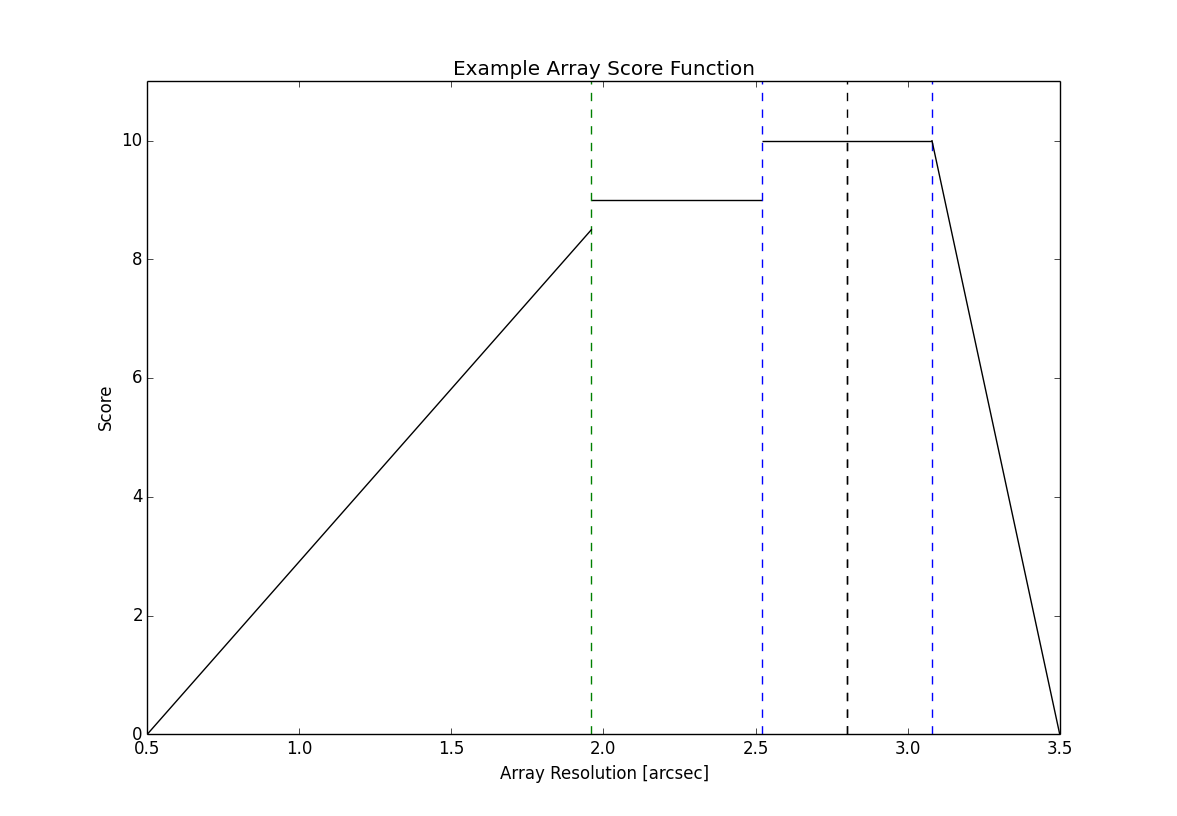
\includegraphics{figure_1.png}}
\caption{In this example, the requested array resolution (\(\rm{SB}_{\rm{AR}}\))
is 2.8 arcsec, with a minimun acceptable resolution
\(\rm{SB}_{\rm{minAR}} = 0.5\) and maximum
\(\rm{SB}_{\rm{maxAR}} = 3.5\)}\end{figure}

\item {} 
\textbf{SB Executive Score}
\phantomsection\label{algorithm:equation-exscore}\begin{gather}
\begin{split}\rm{Score}_{\rm{executive}} = 10; \rm{default\ to\ all\ executives}\end{split}\label{algorithm-exscore}
\end{gather}
\item {} 
\textbf{SB Condition Score}
\phantomsection\label{algorithm:equation-frac_und_1}\begin{gather}
\begin{split}\rm{Score}_{\rm{cond}} = 10 \left(1- (\rm{frac}-1)^{2}\right) \rm{pwv}_{\rm{close}}\end{split}\label{algorithm-frac_und_1}
\end{gather}\phantomsection\label{algorithm:equation-pwv_close}\begin{gather}
\begin{split}\rm{pwv}_{\rm{close}} = 1 - \left|\frac{\rm{pwv} - \rm{maxPWV}}{6}\right|\end{split}\label{algorithm-pwv_close}
\end{gather}\phantomsection\label{algorithm:equation-frac_1}\begin{gather}
\begin{split}\rm{Score}_{\rm{cond}} = 10\end{split}\label{algorithm-frac_1}
\end{gather}
\item {} 
\textbf{SB Total Score}

\end{enumerate}


\section{Checking observability}
\label{algorithm:checking-observability}\label{algorithm:check-obs}

\chapter{Playing with the libraries}
\label{play:playing-with-the-libraries}\label{play::doc}
Load the environment and start ipython:

\begin{Verbatim}[commandchars=\\\{\}]
. activateC2Test
ipython
\end{Verbatim}

Once in ipython::

\begin{Verbatim}[commandchars=\\\{\}]
\PYG{g+gp}{\PYGZgt{}\PYGZgt{}\PYGZgt{} }\PYG{k+kn}{import} \PYG{n+nn}{wtoAlgorithm} \PYG{k+kn}{as} \PYG{n+nn}{wto}
\PYG{g+gp}{\PYGZgt{}\PYGZgt{}\PYGZgt{} }\PYG{k+kn}{import} \PYG{n+nn}{ephem}
\PYG{g+gp}{\PYGZgt{}\PYGZgt{}\PYGZgt{} }\PYG{k+kn}{import} \PYG{n+nn}{pandas} \PYG{k+kn}{as} \PYG{n+nn}{pd}
\PYG{g+gp}{\PYGZgt{}\PYGZgt{}\PYGZgt{} }\PYG{n}{datas} \PYG{o}{=} \PYG{n}{wto}\PYG{o}{.}\PYG{n}{Algorithm}\PYG{p}{(}\PYG{n}{path}\PYG{o}{=}\PYG{l+s}{\PYGZsq{}}\PYG{l+s}{./wto\PYGZus{}testing/}\PYG{l+s}{\PYGZsq{}}\PYG{p}{)}
\end{Verbatim}

And the run the following script. You can copy the code, and then paste into
python with \textbf{\%paste}, or \code{donwload the file},
and then load the function with \textbf{execfile(`runwto.py')}:
\begin{quote}

\begin{Verbatim}[commandchars=\\\{\}]
\PYG{k}{def} \PYG{n+nf}{runwto}\PYG{p}{(}\PYG{n}{pwv}\PYG{p}{,} \PYG{n}{array\PYGZus{}name}\PYG{o}{=}\PYG{n+nb+bp}{None}\PYG{p}{,} \PYG{n}{d}\PYG{o}{=}\PYG{n+nb+bp}{None}\PYG{p}{,} \PYG{n}{num\PYGZus{}ant}\PYG{o}{=}\PYG{l+m+mi}{34}\PYG{p}{)}\PYG{p}{:}
    \PYG{n}{datas}\PYG{o}{.}\PYG{n}{query\PYGZus{}arrays}\PYG{p}{(}\PYG{p}{)}
    \PYG{k}{if} \PYG{n}{array\PYGZus{}name} \PYG{o}{==} \PYG{l+s}{\PYGZsq{}}\PYG{l+s}{default}\PYG{l+s}{\PYGZsq{}}\PYG{p}{:}
        \PYG{n}{array\PYGZus{}name} \PYG{o}{=} \PYG{n+nb+bp}{None}
        \PYG{n}{datas}\PYG{o}{.}\PYG{n}{set\PYGZus{}bl\PYGZus{}prop}\PYG{p}{(}\PYG{n}{array\PYGZus{}name}\PYG{p}{)}
    \PYG{k}{else}\PYG{p}{:}
        \PYG{n}{array\PYGZus{}name} \PYG{o}{=} \PYG{n}{datas}\PYG{o}{.}\PYG{n}{bl\PYGZus{}arrays}\PYG{o}{.}\PYG{n}{AV1}\PYG{o}{.}\PYG{n}{values}\PYG{p}{[}\PYG{l+m+mi}{0}\PYG{p}{]}
        \PYG{n}{datas}\PYG{o}{.}\PYG{n}{set\PYGZus{}bl\PYGZus{}prop}\PYG{p}{(}\PYG{n}{array\PYGZus{}name}\PYG{p}{)}
        \PYG{n}{datas}\PYG{o}{.}\PYG{n}{array\PYGZus{}ar} \PYG{o}{=} \PYG{l+m+mi}{61800} \PYG{o}{/} \PYG{p}{(}\PYG{l+m+mf}{100.} \PYG{o}{*} \PYG{n}{datas}\PYG{o}{.}\PYG{n}{ruv}\PYG{o}{.}\PYG{n}{max}\PYG{p}{(}\PYG{p}{)}\PYG{p}{)}
    \PYG{k}{if} \PYG{n}{d} \PYG{o}{==} \PYG{n+nb+bp}{None}\PYG{p}{:}
        \PYG{n}{d} \PYG{o}{=} \PYG{n}{ephem}\PYG{o}{.}\PYG{n}{now}\PYG{p}{(}\PYG{p}{)}
    \PYG{k}{if} \PYG{n}{num\PYGZus{}ant} \PYG{o}{!=} \PYG{l+m+mi}{34}\PYG{p}{:}
        \PYG{n}{datas}\PYG{o}{.}\PYG{n}{num\PYGZus{}ant} \PYG{o}{=} \PYG{n}{num\PYGZus{}ant}
    \PYG{n}{datas}\PYG{o}{.}\PYG{n}{array\PYGZus{}name} \PYG{o}{=} \PYG{n}{array\PYGZus{}name}
    \PYG{n}{datas}\PYG{o}{.}\PYG{n}{update}\PYG{p}{(}\PYG{p}{)}
    \PYG{n}{datas}\PYG{o}{.}\PYG{n}{date} \PYG{o}{=} \PYG{n}{d}
    \PYG{n}{datas}\PYG{o}{.}\PYG{n}{pwv} \PYG{o}{=} \PYG{n}{pwv}
    \PYG{n}{datas}\PYG{o}{.}\PYG{n}{selector}\PYG{p}{(}\PYG{l+s}{\PYGZsq{}}\PYG{l+s}{12m}\PYG{l+s}{\PYGZsq{}}\PYG{p}{)}
    \PYG{n}{datas}\PYG{o}{.}\PYG{n}{scorer}\PYG{p}{(}\PYG{l+s}{\PYGZsq{}}\PYG{l+s}{12m}\PYG{l+s}{\PYGZsq{}}\PYG{p}{)}
    \PYG{k}{print} \PYG{n}{datas}\PYG{o}{.}\PYG{n}{score12m}\PYG{o}{.}\PYG{n}{sort}\PYG{p}{(}
        \PYG{l+s}{\PYGZsq{}}\PYG{l+s}{score}\PYG{l+s}{\PYGZsq{}}\PYG{p}{,} \PYG{n}{ascending}\PYG{o}{=}\PYG{n+nb+bp}{False}\PYG{p}{)}\PYG{o}{.}\PYG{n}{query}\PYG{p}{(}
        \PYG{l+s}{\PYGZsq{}}\PYG{l+s}{band != }\PYG{l+s}{\PYGZdq{}}\PYG{l+s}{ALMA\PYGZus{}RB\PYGZus{}04}\PYG{l+s}{\PYGZdq{}}\PYG{l+s}{ and band }\PYG{l+s}{\PYGZsq{}}
        \PYG{l+s}{\PYGZsq{}}\PYG{l+s}{!= }\PYG{l+s}{\PYGZdq{}}\PYG{l+s}{ALMA\PYGZus{}RB\PYGZus{}08}\PYG{l+s}{\PYGZdq{}}\PYG{l+s}{ and isPolarization == False}\PYG{l+s}{\PYGZsq{}}\PYG{p}{)}\PYG{p}{[}
        \PYG{p}{[}\PYG{l+s}{\PYGZsq{}}\PYG{l+s}{score}\PYG{l+s}{\PYGZsq{}}\PYG{p}{,}\PYG{l+s}{\PYGZsq{}}\PYG{l+s}{CODE}\PYG{l+s}{\PYGZsq{}}\PYG{p}{,}\PYG{l+s}{\PYGZsq{}}\PYG{l+s}{SB\PYGZus{}UID}\PYG{l+s}{\PYGZsq{}}\PYG{p}{,}\PYG{l+s}{\PYGZsq{}}\PYG{l+s}{name}\PYG{l+s}{\PYGZsq{}}\PYG{p}{,}\PYG{l+s}{\PYGZsq{}}\PYG{l+s}{SB\PYGZus{}state}\PYG{l+s}{\PYGZsq{}}\PYG{p}{,}\PYG{l+s}{\PYGZsq{}}\PYG{l+s}{band}\PYG{l+s}{\PYGZsq{}}\PYG{p}{,}\PYG{l+s}{\PYGZsq{}}\PYG{l+s}{maxPWVC}\PYG{l+s}{\PYGZsq{}}\PYG{p}{,} \PYG{l+s}{\PYGZsq{}}\PYG{l+s}{HA}\PYG{l+s}{\PYGZsq{}}\PYG{p}{,}
         \PYG{l+s}{\PYGZsq{}}\PYG{l+s}{elev}\PYG{l+s}{\PYGZsq{}}\PYG{p}{,}\PYG{l+s}{\PYGZsq{}}\PYG{l+s}{etime}\PYG{l+s}{\PYGZsq{}}\PYG{p}{,} \PYG{l+s}{\PYGZsq{}}\PYG{l+s}{execount}\PYG{l+s}{\PYGZsq{}}\PYG{p}{,}\PYG{l+s}{\PYGZsq{}}\PYG{l+s}{Total}\PYG{l+s}{\PYGZsq{}}\PYG{p}{,}\PYG{l+s}{\PYGZsq{}}\PYG{l+s}{arrayMinAR}\PYG{l+s}{\PYGZsq{}}\PYG{p}{,}\PYG{l+s}{\PYGZsq{}}\PYG{l+s}{arcorr}\PYG{l+s}{\PYGZsq{}}\PYG{p}{,}
         \PYG{l+s}{\PYGZsq{}}\PYG{l+s}{arrayMaxAR}\PYG{l+s}{\PYGZsq{}}\PYG{p}{,}\PYG{l+s}{\PYGZsq{}}\PYG{l+s}{tsysfrac}\PYG{l+s}{\PYGZsq{}}\PYG{p}{,} \PYG{l+s}{\PYGZsq{}}\PYG{l+s}{blfrac}\PYG{l+s}{\PYGZsq{}}\PYG{p}{,}\PYG{l+s}{\PYGZsq{}}\PYG{l+s}{frac}\PYG{l+s}{\PYGZsq{}}\PYG{p}{,}\PYG{l+s}{\PYGZsq{}}\PYG{l+s}{sb\PYGZus{}array\PYGZus{}score}\PYG{l+s}{\PYGZsq{}}\PYG{p}{,}
         \PYG{l+s}{\PYGZsq{}}\PYG{l+s}{sb\PYGZus{}cond\PYGZus{}score}\PYG{l+s}{\PYGZsq{}}\PYG{p}{,} \PYG{l+s}{\PYGZsq{}}\PYG{l+s}{DEC}\PYG{l+s}{\PYGZsq{}}\PYG{p}{,}\PYG{l+s}{\PYGZsq{}}\PYG{l+s}{RA}\PYG{l+s}{\PYGZsq{}}\PYG{p}{,} \PYG{l+s}{\PYGZsq{}}\PYG{l+s}{isTimeConstrained}\PYG{l+s}{\PYGZsq{}}\PYG{p}{,}
         \PYG{l+s}{\PYGZsq{}}\PYG{l+s}{integrationTime}\PYG{l+s}{\PYGZsq{}}\PYG{p}{,} \PYG{l+s}{\PYGZsq{}}\PYG{l+s}{PRJ\PYGZus{}ARCHIVE\PYGZus{}UID}\PYG{l+s}{\PYGZsq{}}\PYG{p}{]}\PYG{p}{]}\PYG{o}{.}\PYG{n}{head}\PYG{p}{(}\PYG{l+m+mi}{25}\PYG{p}{)}
    \PYG{n}{datas}\PYG{o}{.}\PYG{n}{num\PYGZus{}ant\PYGZus{}user} \PYG{o}{=} \PYG{l+m+mi}{34}
\end{Verbatim}
\end{quote}

The to run the wto algorithm use a pwv value between 0 and 20, with steps of
0.05 (e.g., 0.4, 0.45, but no 0.42), and assuming the latest BL Array. Set
\code{array\_name='default'} when running \code{runwto} (e.g.
\code{runwto(X.XX, array\_name='default')}) to use the Current configuration parameters
calculated with arrayConfigurationTools and 34 antennas. Also, to change the
date to current date use \code{runwto(X.XX, d=ephem.Date('2014-06-28 03:45')}

This will display the top 25 values of datas.scorer12m dataFrame. To check full
output in an excel table run::

\begin{Verbatim}[commandchars=\\\{\}]
\PYG{n}{datas}\PYG{o}{.}\PYG{n}{score12m}\PYG{o}{.}\PYG{n}{to\PYGZus{}excel}\PYG{p}{(}\PYG{l+s}{\PYGZsq{}}\PYG{l+s}{output\PYGZus{}path/score.xls}\PYG{l+s}{\PYGZsq{}}\PYG{p}{)}
\end{Verbatim}

Where output\_path is the full path to the directory where you want to save the
score.xls excel spreadsheet.


\chapter{The WTO API}
\label{wtoapi::doc}\label{wtoapi:the-wto-api}\label{wtoapi:module-wtoDatabase}\index{wtoDatabase (module)}

\section{wtoDatabase.py: the gWTO database library.}
\label{wtoapi:wtodatabase-py-the-gwto-database-library}
This library contains the classes and functions required to query, parse and
organize the Projects and SchedBlock information stored at the OSF archive in
different tables.
\index{ObsProject (class in wtoDatabase)}

\begin{fulllineitems}
\phantomsection\label{wtoapi:wtoDatabase.ObsProject}\pysiglinewithargsret{\strong{class }\code{wtoDatabase.}\bfcode{ObsProject}}{\emph{xml\_file}, \emph{path='./'}}{}~\begin{quote}\begin{description}
\item[{Parameters}] \leavevmode\begin{itemize}
\item {} 
\textbf{xml\_file} -- 

\item {} 
\textbf{path} -- 

\end{itemize}

\end{description}\end{quote}
\index{assoc\_sched\_blocks() (wtoDatabase.ObsProject method)}

\begin{fulllineitems}
\phantomsection\label{wtoapi:wtoDatabase.ObsProject.assoc_sched_blocks}\pysiglinewithargsret{\bfcode{assoc\_sched\_blocks}}{}{}~\begin{quote}\begin{description}
\item[{Returns}] \leavevmode


\end{description}\end{quote}

\end{fulllineitems}


\end{fulllineitems}

\index{WtoDatabase (class in wtoDatabase)}

\begin{fulllineitems}
\phantomsection\label{wtoapi:wtoDatabase.WtoDatabase}\pysiglinewithargsret{\strong{class }\code{wtoDatabase.}\bfcode{WtoDatabase}}{\emph{path='/.wto/'}, \emph{source=None}, \emph{forcenew=False}}{}
WtoDatabase is the class that stores the Projects and SB information in
dataframes, and it also has the methods to connect and query the OSF
archive for this info.

A default instance will use the directory \$HOME/.wto as a cache, and by
default find the approved Cycle 2 projects and carried-over Cycle 1
projects. If a file name or list are given as `source' parameter, only the
information of the projects in that list or filename will be ingested.

Setting \emph{forcenew} to True will force the cleaning of the cache dir, and
all information will be processed again.
\begin{quote}\begin{description}
\item[{Parameters}] \leavevmode\begin{itemize}
\item {} 
\textbf{path} (\emph{str, default `\$HOME/.wto'}) -- Path for data cache.

\item {} 
\textbf{source} (\emph{list or str}) -- File or list of strings with the codes of the projects
to be ingested by WtoDatabase.

\item {} 
\textbf{forcenew} (\emph{boolean, default False}) -- Force cache cleaning and reload from archive.

\end{itemize}

\end{description}\end{quote}
\index{create\_allsb() (wtoDatabase.WtoDatabase method)}

\begin{fulllineitems}
\phantomsection\label{wtoapi:wtoDatabase.WtoDatabase.create_allsb}\pysiglinewithargsret{\bfcode{create\_allsb}}{\emph{split=False}, \emph{path=None}}{}~\begin{quote}\begin{description}
\item[{Parameters}] \leavevmode\begin{itemize}
\item {} 
\textbf{split} -- 

\item {} 
\textbf{path} -- 

\end{itemize}

\end{description}\end{quote}

\end{fulllineitems}

\index{create\_summary() (wtoDatabase.WtoDatabase method)}

\begin{fulllineitems}
\phantomsection\label{wtoapi:wtoDatabase.WtoDatabase.create_summary}\pysiglinewithargsret{\bfcode{create\_summary}}{}{}
\end{fulllineitems}

\index{filter\_c1() (wtoDatabase.WtoDatabase method)}

\begin{fulllineitems}
\phantomsection\label{wtoapi:wtoDatabase.WtoDatabase.filter_c1}\pysiglinewithargsret{\bfcode{filter\_c1}}{}{}
\end{fulllineitems}

\index{forcenew() (wtoDatabase.WtoDatabase method)}

\begin{fulllineitems}
\phantomsection\label{wtoapi:wtoDatabase.WtoDatabase.forcenew}\pysiglinewithargsret{\bfcode{forcenew}}{}{}
\end{fulllineitems}

\index{get\_obsproject() (wtoDatabase.WtoDatabase method)}

\begin{fulllineitems}
\phantomsection\label{wtoapi:wtoDatabase.WtoDatabase.get_obsproject}\pysiglinewithargsret{\bfcode{get\_obsproject}}{\emph{code}}{}~\begin{quote}\begin{description}
\item[{Parameters}] \leavevmode
\textbf{code} -- 

\end{description}\end{quote}

\end{fulllineitems}

\index{populate\_newar() (wtoDatabase.WtoDatabase method)}

\begin{fulllineitems}
\phantomsection\label{wtoapi:wtoDatabase.WtoDatabase.populate_newar}\pysiglinewithargsret{\bfcode{populate\_newar}}{}{}
\end{fulllineitems}

\index{populate\_schedblock\_info() (wtoDatabase.WtoDatabase method)}

\begin{fulllineitems}
\phantomsection\label{wtoapi:wtoDatabase.WtoDatabase.populate_schedblock_info}\pysiglinewithargsret{\bfcode{populate\_schedblock\_info}}{}{}
\end{fulllineitems}

\index{populate\_schedblocks() (wtoDatabase.WtoDatabase method)}

\begin{fulllineitems}
\phantomsection\label{wtoapi:wtoDatabase.WtoDatabase.populate_schedblocks}\pysiglinewithargsret{\bfcode{populate\_schedblocks}}{}{}
\end{fulllineitems}

\index{populate\_sciencegoals\_sbxml() (wtoDatabase.WtoDatabase method)}

\begin{fulllineitems}
\phantomsection\label{wtoapi:wtoDatabase.WtoDatabase.populate_sciencegoals_sbxml}\pysiglinewithargsret{\bfcode{populate\_sciencegoals\_sbxml}}{}{}
\end{fulllineitems}

\index{row\_fieldsource() (wtoDatabase.WtoDatabase method)}

\begin{fulllineitems}
\phantomsection\label{wtoapi:wtoDatabase.WtoDatabase.row_fieldsource}\pysiglinewithargsret{\bfcode{row\_fieldsource}}{\emph{fs}, \emph{sbuid}, \emph{array}, \emph{new=False}}{}~\begin{quote}\begin{description}
\item[{Parameters}] \leavevmode\begin{itemize}
\item {} 
\textbf{fs} -- 

\item {} 
\textbf{sbuid} -- 

\item {} 
\textbf{new} -- 

\end{itemize}

\end{description}\end{quote}

\end{fulllineitems}

\index{row\_newar() (wtoDatabase.WtoDatabase method)}

\begin{fulllineitems}
\phantomsection\label{wtoapi:wtoDatabase.WtoDatabase.row_newar}\pysiglinewithargsret{\bfcode{row\_newar}}{\emph{sbuid}, \emph{new=False}}{}~\begin{quote}\begin{description}
\item[{Parameters}] \leavevmode\begin{itemize}
\item {} 
\textbf{sbuid} -- 

\item {} 
\textbf{new} -- 

\end{itemize}

\end{description}\end{quote}

\end{fulllineitems}

\index{row\_schedblock\_info() (wtoDatabase.WtoDatabase method)}

\begin{fulllineitems}
\phantomsection\label{wtoapi:wtoDatabase.WtoDatabase.row_schedblock_info}\pysiglinewithargsret{\bfcode{row\_schedblock\_info}}{\emph{sb\_uid}, \emph{new=False}}{}~\begin{quote}\begin{description}
\item[{Parameters}] \leavevmode\begin{itemize}
\item {} 
\textbf{sb\_uid} -- 

\item {} 
\textbf{new} -- 

\end{itemize}

\end{description}\end{quote}

\end{fulllineitems}

\index{row\_schedblocks() (wtoDatabase.WtoDatabase method)}

\begin{fulllineitems}
\phantomsection\label{wtoapi:wtoDatabase.WtoDatabase.row_schedblocks}\pysiglinewithargsret{\bfcode{row\_schedblocks}}{\emph{sb\_uid}, \emph{partid}, \emph{new=False}}{}~\begin{quote}\begin{description}
\item[{Parameters}] \leavevmode\begin{itemize}
\item {} 
\textbf{sb\_uid} -- 

\item {} 
\textbf{partid} -- 

\item {} 
\textbf{new} -- 

\end{itemize}

\end{description}\end{quote}

\end{fulllineitems}

\index{row\_sciencegoals() (wtoDatabase.WtoDatabase method)}

\begin{fulllineitems}
\phantomsection\label{wtoapi:wtoDatabase.WtoDatabase.row_sciencegoals}\pysiglinewithargsret{\bfcode{row\_sciencegoals}}{\emph{code}, \emph{new=False}}{}~\begin{quote}\begin{description}
\item[{Parameters}] \leavevmode\begin{itemize}
\item {} 
\textbf{code} -- 

\item {} 
\textbf{new} -- 

\end{itemize}

\item[{Returns}] \leavevmode


\end{description}\end{quote}

\end{fulllineitems}

\index{row\_spectralconf() (wtoDatabase.WtoDatabase method)}

\begin{fulllineitems}
\phantomsection\label{wtoapi:wtoDatabase.WtoDatabase.row_spectralconf}\pysiglinewithargsret{\bfcode{row\_spectralconf}}{\emph{ss}, \emph{sbuid}, \emph{new=False}}{}~\begin{quote}\begin{description}
\item[{Parameters}] \leavevmode\begin{itemize}
\item {} 
\textbf{ss} -- 

\item {} 
\textbf{sbuid} -- 

\item {} 
\textbf{new} -- 

\end{itemize}

\end{description}\end{quote}

\end{fulllineitems}

\index{row\_target() (wtoDatabase.WtoDatabase method)}

\begin{fulllineitems}
\phantomsection\label{wtoapi:wtoDatabase.WtoDatabase.row_target}\pysiglinewithargsret{\bfcode{row\_target}}{\emph{tg}, \emph{sbuid}, \emph{new=False}}{}~\begin{quote}\begin{description}
\item[{Parameters}] \leavevmode\begin{itemize}
\item {} 
\textbf{tg} -- 

\item {} 
\textbf{sbuid} -- 

\item {} 
\textbf{new} -- 

\end{itemize}

\end{description}\end{quote}

\end{fulllineitems}

\index{start\_wto() (wtoDatabase.WtoDatabase method)}

\begin{fulllineitems}
\phantomsection\label{wtoapi:wtoDatabase.WtoDatabase.start_wto}\pysiglinewithargsret{\bfcode{start\_wto}}{}{}
Initializes the wtoDatabase dataframes.

The function queries the archive to look for cycle 1 and cycle 2
projects, disregarding any projects with status ``Approved'',
``Phase1Submitted'', ``Broken'', ``Canceled'' or ``Rejected''.

The archive tables used are ALMA.BMMV\_OBSPROPOSAL,
ALMA.OBS\_PROJECT\_STATUS, ALMA.BMMV\_OBSPROJECT and
ALMA.XML\_OBSPROJECT\_ENTITIES.
\begin{quote}\begin{description}
\item[{Returns}] \leavevmode
None

\end{description}\end{quote}

\end{fulllineitems}

\index{update() (wtoDatabase.WtoDatabase method)}

\begin{fulllineitems}
\phantomsection\label{wtoapi:wtoDatabase.WtoDatabase.update}\pysiglinewithargsret{\bfcode{update}}{\emph{connect=True}}{}~\begin{quote}\begin{description}
\item[{Parameters}] \leavevmode
\textbf{connect} -- 

\item[{Returns}] \leavevmode


\end{description}\end{quote}

\end{fulllineitems}


\end{fulllineitems}

\index{convert\_deg() (in module wtoDatabase)}

\begin{fulllineitems}
\phantomsection\label{wtoapi:wtoDatabase.convert_deg}\pysiglinewithargsret{\code{wtoDatabase.}\bfcode{convert\_deg}}{\emph{angle}, \emph{unit}}{}~\begin{quote}\begin{description}
\item[{Parameters}] \leavevmode\begin{itemize}
\item {} 
\textbf{angle} -- 

\item {} 
\textbf{unit} -- 

\end{itemize}

\item[{Returns}] \leavevmode


\end{description}\end{quote}

\end{fulllineitems}

\index{convert\_ghz() (in module wtoDatabase)}

\begin{fulllineitems}
\phantomsection\label{wtoapi:wtoDatabase.convert_ghz}\pysiglinewithargsret{\code{wtoDatabase.}\bfcode{convert\_ghz}}{\emph{freq}, \emph{unit}}{}~\begin{quote}\begin{description}
\item[{Parameters}] \leavevmode\begin{itemize}
\item {} 
\textbf{freq} -- 

\item {} 
\textbf{unit} -- 

\end{itemize}

\item[{Returns}] \leavevmode


\end{description}\end{quote}

\end{fulllineitems}

\index{convert\_jy() (in module wtoDatabase)}

\begin{fulllineitems}
\phantomsection\label{wtoapi:wtoDatabase.convert_jy}\pysiglinewithargsret{\code{wtoDatabase.}\bfcode{convert\_jy}}{\emph{flux}, \emph{unit}}{}~\begin{quote}\begin{description}
\item[{Parameters}] \leavevmode\begin{itemize}
\item {} 
\textbf{flux} -- 

\item {} 
\textbf{unit} -- 

\end{itemize}

\item[{Returns}] \leavevmode


\end{description}\end{quote}

\end{fulllineitems}

\index{convert\_mjy() (in module wtoDatabase)}

\begin{fulllineitems}
\phantomsection\label{wtoapi:wtoDatabase.convert_mjy}\pysiglinewithargsret{\code{wtoDatabase.}\bfcode{convert\_mjy}}{\emph{flux}, \emph{unit}}{}~\begin{quote}\begin{description}
\item[{Parameters}] \leavevmode\begin{itemize}
\item {} 
\textbf{flux} -- 

\item {} 
\textbf{unit} -- 

\end{itemize}

\item[{Returns}] \leavevmode


\end{description}\end{quote}

\end{fulllineitems}

\index{convert\_sec() (in module wtoDatabase)}

\begin{fulllineitems}
\phantomsection\label{wtoapi:wtoDatabase.convert_sec}\pysiglinewithargsret{\code{wtoDatabase.}\bfcode{convert\_sec}}{\emph{angle}, \emph{unit}}{}~\begin{quote}\begin{description}
\item[{Parameters}] \leavevmode\begin{itemize}
\item {} 
\textbf{angle} -- 

\item {} 
\textbf{unit} -- 

\end{itemize}

\item[{Returns}] \leavevmode


\end{description}\end{quote}

\end{fulllineitems}

\index{convert\_tsec() (in module wtoDatabase)}

\begin{fulllineitems}
\phantomsection\label{wtoapi:wtoDatabase.convert_tsec}\pysiglinewithargsret{\code{wtoDatabase.}\bfcode{convert\_tsec}}{\emph{time}, \emph{unit}}{}~\begin{quote}\begin{description}
\item[{Parameters}] \leavevmode\begin{itemize}
\item {} 
\textbf{time} -- 

\item {} 
\textbf{unit} -- 

\end{itemize}

\item[{Returns}] \leavevmode


\end{description}\end{quote}

\end{fulllineitems}

\phantomsection\label{wtoapi:module-wtoAlgorithm}\index{wtoAlgorithm (module)}

\section{wtoAlgorithm.py: the gWTO selector and scorer library.}
\label{wtoapi:wtoalgorithm-py-the-gwto-selector-and-scorer-library}
This library contains the classes and functions required to select and rank
SBs from the information that is stored in a WtoDatabse object.
\index{WtoAlgorithm (class in wtoAlgorithm)}

\begin{fulllineitems}
\phantomsection\label{wtoapi:wtoAlgorithm.WtoAlgorithm}\pysiglinewithargsret{\strong{class }\code{wtoAlgorithm.}\bfcode{WtoAlgorithm}}{\emph{path='/.wto/'}, \emph{source=None}, \emph{forcenew=False}}{}
Inherits from WtoDatabase, adds the methods for selection and scoring.
It also sets the default parameters for these methods: pwv=1.2, date=now,
array angular resolution, transmission=0.5, minha=-5, maxha=3, etc.
\begin{quote}\begin{description}
\item[{Parameters}] \leavevmode\begin{itemize}
\item {} 
\textbf{path} (\emph{(default='/.wto/') String.}) -- A path, relative to \$HOME, where the cache is stored.

\item {} 
\textbf{source} -- See WtoDatabase definitions.

\item {} 
\textbf{forcenew} -- See WtoDatabase definitions.

\end{itemize}

\item[{Returns}] \leavevmode
A WtoAlgorithm instance.

\end{description}\end{quote}
\index{calculate\_score() (wtoAlgorithm.WtoAlgorithm method)}

\begin{fulllineitems}
\phantomsection\label{wtoapi:wtoAlgorithm.WtoAlgorithm.calculate_score}\pysiglinewithargsret{\bfcode{calculate\_score}}{\emph{ecount}, \emph{tcount}, \emph{srank}, \emph{ar}, \emph{aminar}, \emph{amaxar}, \emph{las}, \emph{grade}, \emph{repfreq}, \emph{dec}, \emph{execu}, \emph{array}, \emph{frac}, \emph{maxpwvc}, \emph{code}, \emph{points}}{}
Please go to the {\hyperref[algorithm:score]{\emph{Score and ranking}}} (\autopageref*{algorithm:score}) section for an
algorithm's description.
\begin{quote}\begin{description}
\item[{Parameters}] \leavevmode\begin{itemize}
\item {} 
\textbf{ecount} (\emph{Integer.}) -- Executions requested by the SB

\item {} 
\textbf{tcount} (\emph{Integer.}) -- Total executions with QA0 Pass or Unset for the SB.

\item {} 
\textbf{srank} (\emph{Intenger}) -- SB Science ranking.

\item {} 
\textbf{ar} (\emph{Float.}) -- SB requested Angular Resolution, from the Science Goal.

\item {} 
\textbf{aminar} (\emph{Float. In arcsec.}) -- The minum angular resolution the SB can accept to be
observed.

\item {} 
\textbf{amaxar} (\emph{Float. In arcsec.}) -- The maximum angular resolution the SB can accept to be
observed.

\item {} 
\textbf{las} (\emph{Float. In arcsec.}) -- SB requested Largest Angular Scale, from the Science Goal.

\item {} 
\textbf{grade} (\emph{String, can be A, B or C.}) -- SB's Project letter grade.

\item {} 
\textbf{repfreq} (\emph{Float, in GHz.}) -- SB's representative frequency.

\item {} 
\textbf{dec} (\emph{Float, in degrees.}) -- SB's representative declination coordinates, as determined
by self.check\_observability().

\item {} 
\textbf{execu} (\emph{String, can be NA, EU, EA, CL or OTHER.}) -- SB's Project Executive.

\item {} 
\textbf{array} (\emph{String, can be 12m, 7m or tp.}) -- Array type.

\item {} 
\textbf{frac} (\emph{Float.}) -- Total time fraction calculated by self.selector() for the
SB to reach the required sensitivity.

\item {} 
\textbf{maxpwvc} (\emph{Float, a value between 0 and 20.}) -- SB's maxPWVC variable.

\item {} 
\textbf{code} (\emph{String.}) -- SB's project code.

\end{itemize}

\item[{Returns}] \leavevmode
Tuple with ...

\end{description}\end{quote}

\end{fulllineitems}

\index{check\_observability() (wtoAlgorithm.WtoAlgorithm method)}

\begin{fulllineitems}
\phantomsection\label{wtoapi:wtoAlgorithm.WtoAlgorithm.check_observability}\pysiglinewithargsret{\bfcode{check\_observability}}{\emph{array}}{}~\begin{quote}\begin{description}
\item[{Parameters}] \leavevmode
\textbf{array} -- 

\item[{Returns}] \leavevmode


\end{description}\end{quote}

\end{fulllineitems}

\index{query\_arrays() (wtoAlgorithm.WtoAlgorithm method)}

\begin{fulllineitems}
\phantomsection\label{wtoapi:wtoAlgorithm.WtoAlgorithm.query_arrays}\pysiglinewithargsret{\bfcode{query\_arrays}}{}{}
\end{fulllineitems}

\index{scorer() (wtoAlgorithm.WtoAlgorithm method)}

\begin{fulllineitems}
\phantomsection\label{wtoapi:wtoAlgorithm.WtoAlgorithm.scorer}\pysiglinewithargsret{\bfcode{scorer}}{\emph{array}}{}
Method that handles the score calculation for each array type. It
applies \code{self.calculate\_score()} to the previously selected SBs using
\code{self.selector()}
\begin{quote}\begin{description}
\item[{Parameters}] \leavevmode
\textbf{array} (\emph{String.}) -- `12m', `7m', `tp'

\item[{Returns}] \leavevmode
Creates a score table for the instance, which will be named as
\code{score12m}, \code{score7m} or \code{scoretp}.

\end{description}\end{quote}

\end{fulllineitems}

\index{selector() (wtoAlgorithm.WtoAlgorithm method)}

\begin{fulllineitems}
\phantomsection\label{wtoapi:wtoAlgorithm.WtoAlgorithm.selector}\pysiglinewithargsret{\bfcode{selector}}{\emph{array}}{}
Selects SBs that can be observed given the current weather conditions,
HA range, array type and array configuration (in the case of 12m array
type) and SB/Project Status. See
{\hyperref[algorithm:selection]{\emph{Selection and Data preparation}}} (\autopageref*{algorithm:selection})
\begin{quote}\begin{description}
\item[{Parameters}] \leavevmode
\textbf{array} (\emph{String.}) -- `12m', `7m', `tp'

\item[{Returns}] \leavevmode
Depending on the array type, creates tables select12m, select7m
or selecttp.

\end{description}\end{quote}

\end{fulllineitems}

\index{set\_array\_ar() (wtoAlgorithm.WtoAlgorithm method)}

\begin{fulllineitems}
\phantomsection\label{wtoapi:wtoAlgorithm.WtoAlgorithm.set_array_ar}\pysiglinewithargsret{\bfcode{set\_array\_ar}}{\emph{ar}}{}~\begin{quote}\begin{description}
\item[{Parameters}] \leavevmode
\textbf{ar} -- 

\end{description}\end{quote}

\end{fulllineitems}

\index{set\_arrayar() (wtoAlgorithm.WtoAlgorithm method)}

\begin{fulllineitems}
\phantomsection\label{wtoapi:wtoAlgorithm.WtoAlgorithm.set_arrayar}\pysiglinewithargsret{\bfcode{set\_arrayar}}{\emph{ar}}{}~\begin{quote}\begin{description}
\item[{Parameters}] \leavevmode
\textbf{ar} -- 

\end{description}\end{quote}

\end{fulllineitems}

\index{set\_bl\_prop() (wtoAlgorithm.WtoAlgorithm method)}

\begin{fulllineitems}
\phantomsection\label{wtoapi:wtoAlgorithm.WtoAlgorithm.set_bl_prop}\pysiglinewithargsret{\bfcode{set\_bl\_prop}}{\emph{array\_name}}{}~\begin{quote}\begin{description}
\item[{Parameters}] \leavevmode
\textbf{array\_name} -- 

\end{description}\end{quote}

\end{fulllineitems}

\index{set\_date() (wtoAlgorithm.WtoAlgorithm method)}

\begin{fulllineitems}
\phantomsection\label{wtoapi:wtoAlgorithm.WtoAlgorithm.set_date}\pysiglinewithargsret{\bfcode{set\_date}}{\emph{date}}{}~\begin{quote}\begin{description}
\item[{Parameters}] \leavevmode
\textbf{date} -- 

\end{description}\end{quote}

\end{fulllineitems}

\index{set\_maxha() (wtoAlgorithm.WtoAlgorithm method)}

\begin{fulllineitems}
\phantomsection\label{wtoapi:wtoAlgorithm.WtoAlgorithm.set_maxha}\pysiglinewithargsret{\bfcode{set\_maxha}}{\emph{ha}}{}~\begin{quote}\begin{description}
\item[{Parameters}] \leavevmode
\textbf{ha} -- 

\end{description}\end{quote}

\end{fulllineitems}

\index{set\_minha() (wtoAlgorithm.WtoAlgorithm method)}

\begin{fulllineitems}
\phantomsection\label{wtoapi:wtoAlgorithm.WtoAlgorithm.set_minha}\pysiglinewithargsret{\bfcode{set\_minha}}{\emph{ha}}{}~\begin{quote}\begin{description}
\item[{Parameters}] \leavevmode
\textbf{ha} -- 

\end{description}\end{quote}

\end{fulllineitems}

\index{set\_pwv() (wtoAlgorithm.WtoAlgorithm method)}

\begin{fulllineitems}
\phantomsection\label{wtoapi:wtoAlgorithm.WtoAlgorithm.set_pwv}\pysiglinewithargsret{\bfcode{set\_pwv}}{\emph{pwv}}{}~\begin{quote}\begin{description}
\item[{Parameters}] \leavevmode
\textbf{pwv} -- 

\end{description}\end{quote}

\end{fulllineitems}

\index{set\_trans() (wtoAlgorithm.WtoAlgorithm method)}

\begin{fulllineitems}
\phantomsection\label{wtoapi:wtoAlgorithm.WtoAlgorithm.set_trans}\pysiglinewithargsret{\bfcode{set\_trans}}{\emph{transmission}}{}~\begin{quote}\begin{description}
\item[{Parameters}] \leavevmode
\textbf{transmission} -- 

\end{description}\end{quote}

\end{fulllineitems}


\end{fulllineitems}

\index{observable() (in module wtoAlgorithm)}

\begin{fulllineitems}
\phantomsection\label{wtoapi:wtoAlgorithm.observable}\pysiglinewithargsret{\code{wtoAlgorithm.}\bfcode{observable}}{\emph{solarSystem}, \emph{sourcename}, \emph{RA}, \emph{DEC}, \emph{horizon}, \emph{isQuery}, \emph{ephemeris}, \emph{alma}}{}~\begin{quote}\begin{description}
\item[{Parameters}] \leavevmode\begin{itemize}
\item {} 
\textbf{solarSystem} -- 

\item {} 
\textbf{sourcename} -- 

\item {} 
\textbf{RA} -- 

\item {} 
\textbf{DEC} -- 

\item {} 
\textbf{horizon} -- 

\item {} 
\textbf{isQuery} -- 

\item {} 
\textbf{ephemeris} -- 

\item {} 
\textbf{alma} -- 

\end{itemize}

\item[{Returns}] \leavevmode


\end{description}\end{quote}

\end{fulllineitems}

\index{read\_ephemeris() (in module wtoAlgorithm)}

\begin{fulllineitems}
\phantomsection\label{wtoapi:wtoAlgorithm.read_ephemeris}\pysiglinewithargsret{\code{wtoAlgorithm.}\bfcode{read\_ephemeris}}{\emph{ephemeris}, \emph{date}}{}~\begin{quote}\begin{description}
\item[{Parameters}] \leavevmode\begin{itemize}
\item {} 
\textbf{ephemeris} -- 

\item {} 
\textbf{date} -- 

\end{itemize}

\item[{Returns}] \leavevmode


\end{description}\end{quote}

\end{fulllineitems}

\begin{figure}[htbp]
\centering
\capstart

\scalebox{0.650000}{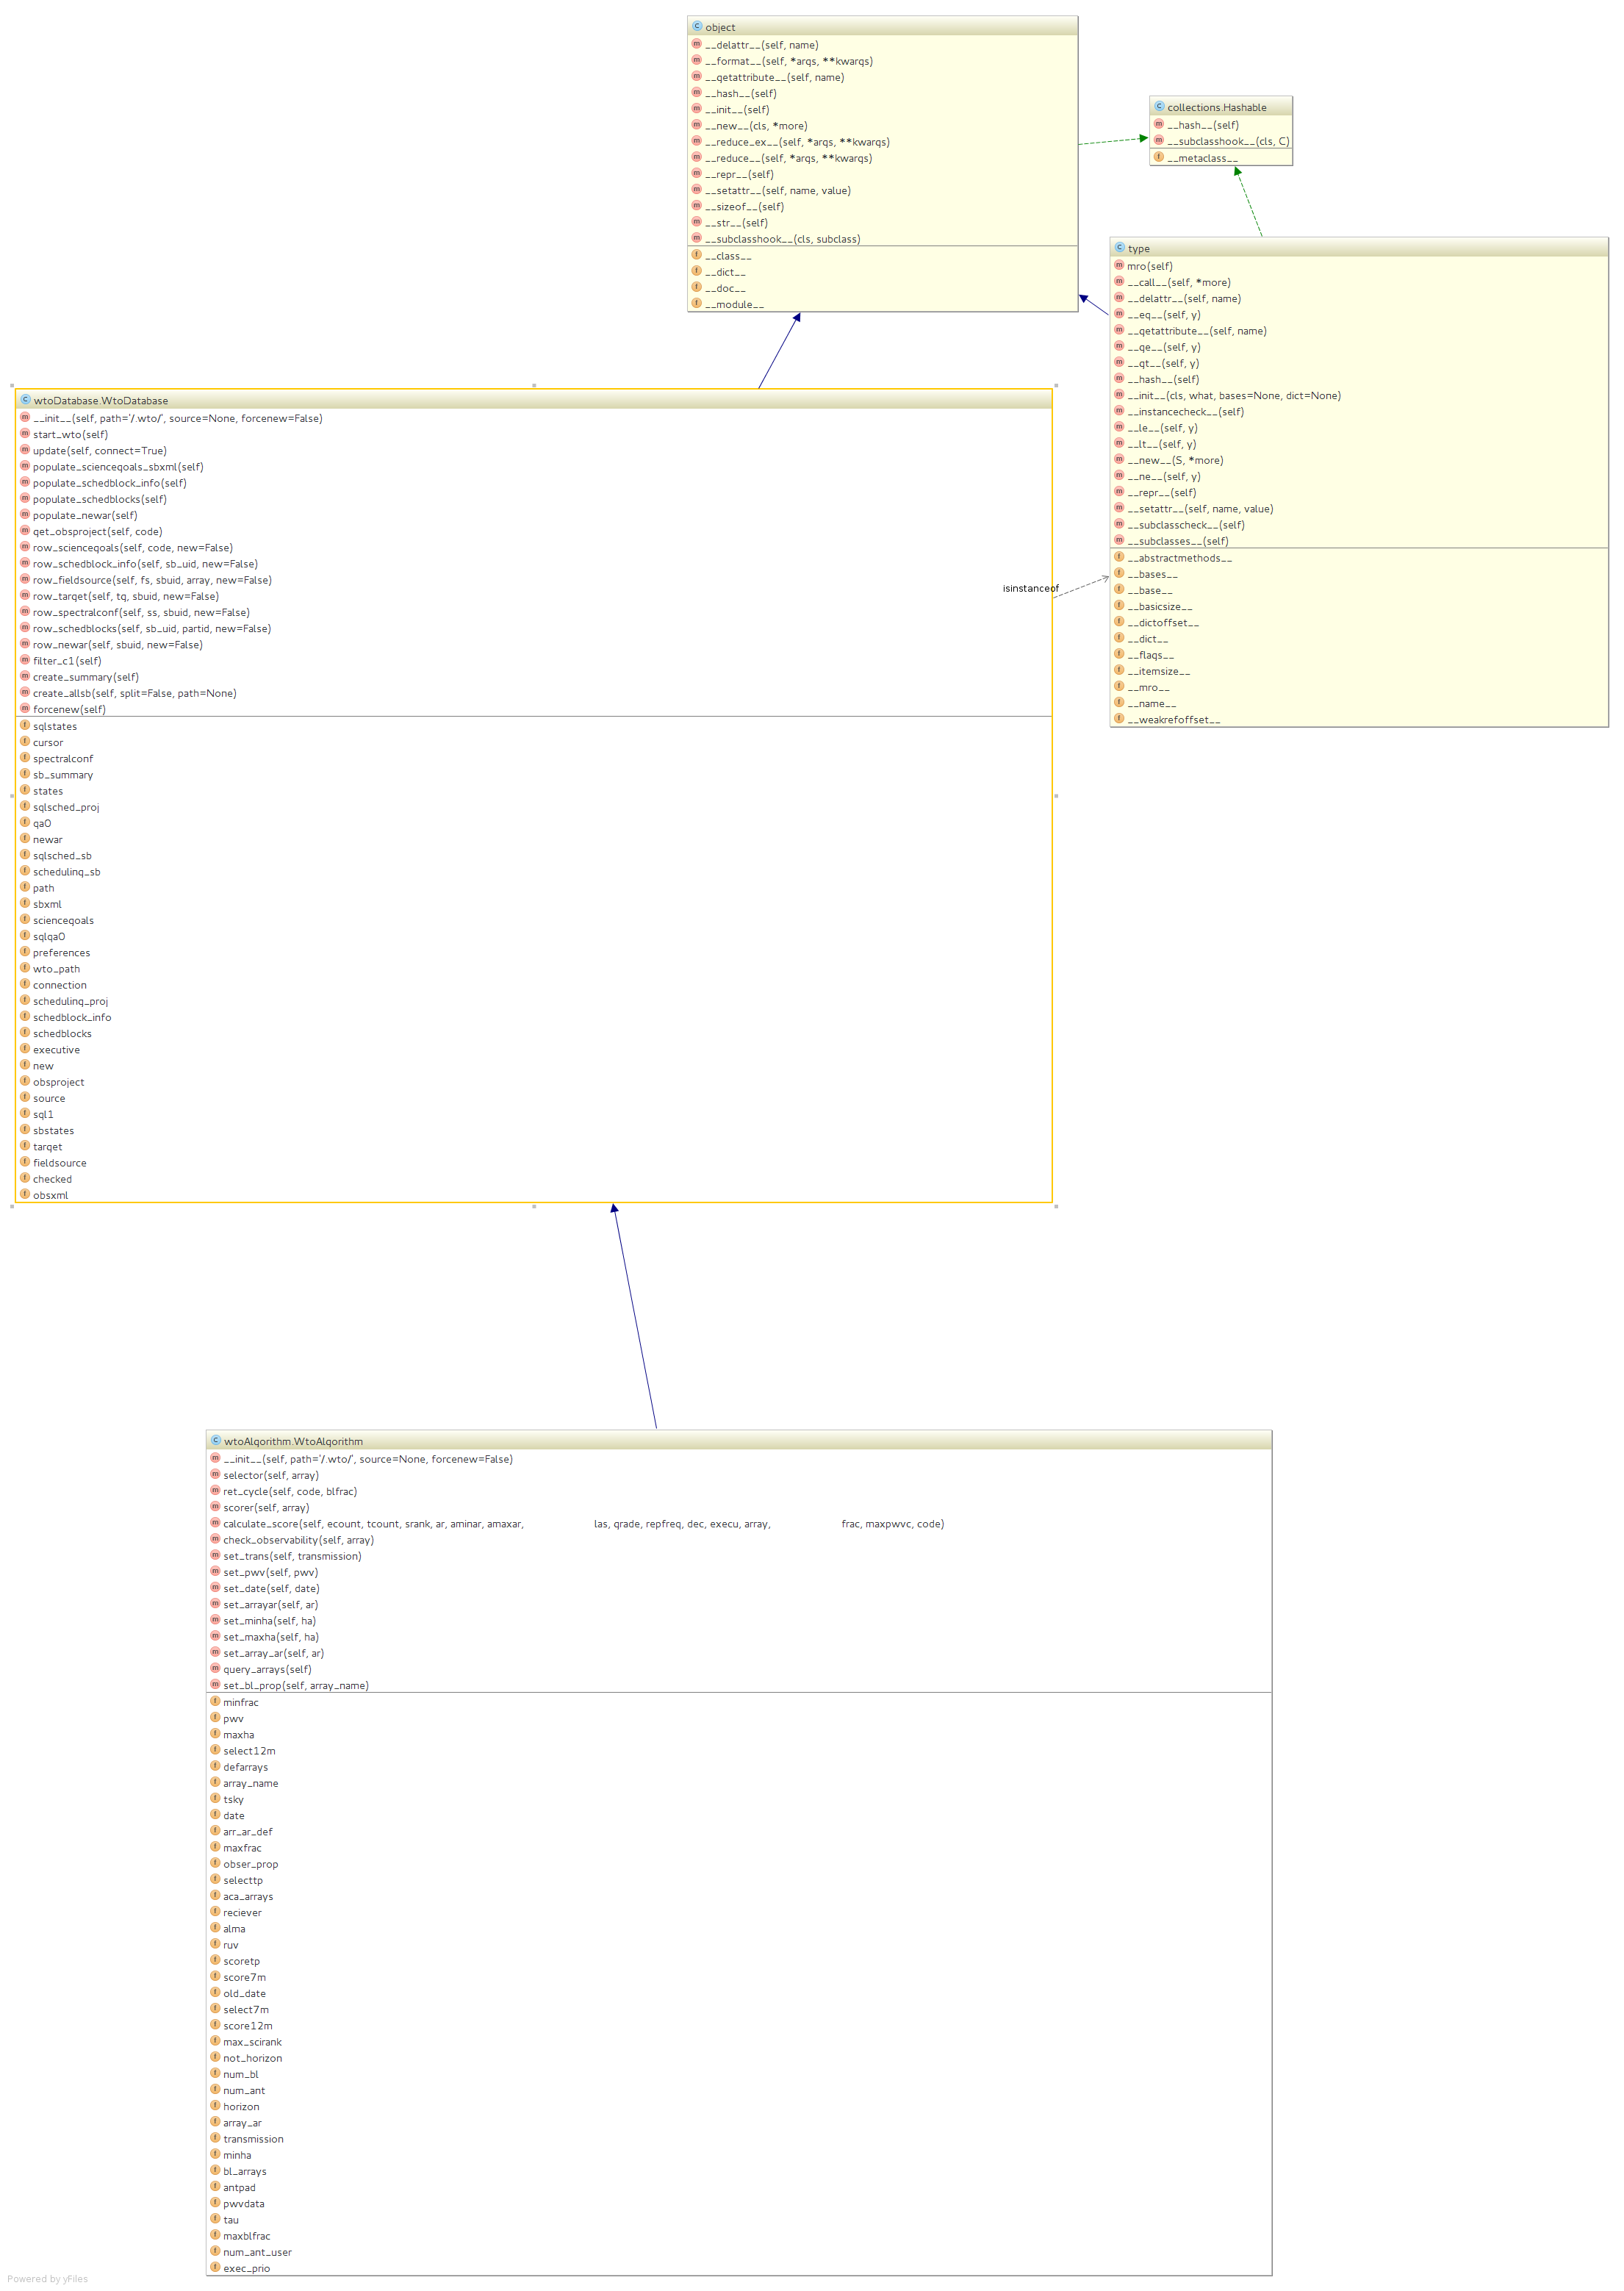
\includegraphics{diagram.png}}
\caption{Figure 4, UML diagram of wtoAlgorithm.py}\end{figure}


\chapter{The WTO Data Frames}
\label{wtodata::doc}\label{wtodata:the-wto-data-frames}

\section{wtoDatabase.obsprojects}
\label{wtodata:wtodatabase-obsprojects}
Main obsproject table ingested from queries to the archive.

\begin{tabulary}{\linewidth}{|L|L|}
\hline
\textsf{\relax 
COLUMN
} & \textsf{\relax 
VALUE
}\\
\hline
PRJ\_ARCHIVE\_UID
 & 
\emph{(string)} Project UID (1)
\\

DELETED
 & 
\emph{(boolean int)} Is Deleted? (2)
\\

PI
 & 
\emph{(string)} Principal Investigator (3)
\\

PRJ\_NAME
 & 
\emph{(string)} Project Name (4)
\\

** CODE
 & 
\emph{(string)} Project Code (5)
\\

PRJ\_TIME\_OF\_CREATION
 & 
\emph{(string)} Project creation timestamp (6)
\\

PRJ\_SCIENTIFIC\_RANK
 & 
\emph{(int64)} Project Rank (7)
\\

PRJ\_VERSION
 & 
\emph{(string)} Project Version (8)
\\

PRJ\_LETTER\_GRADE
 & 
\emph{(string)} Project Grade (9)
\\

DOMAIN\_ENTITY\_STATE
 & 
\emph{(string)} Project Status (10)
\\

OBS\_PROJECT\_ID
 & 
\emph{(string)} Project UID (11)
\\

EXEC
 & 
\emph{(string)} Executive (12)
\\

timestamp
 & 
\emph{(datetime64{[}ns{]})} Project latest update date (13)
\\

obsproj
 & 
\emph{(string)} Obsproject XML filename (14)
\\
\hline\end{tabulary}

\begin{enumerate}
\item {} 
ALMA.BMMV\_OBSPROJECT.PRJ\_ARCHIVE\_UID

\item {} 
ALMA.BMMV\_OBSPROJECT.DELETED

\item {} 
ALMA.BMMV\_OBSPROJECT.PI

\item {} 
ALMA.BMMV\_OBSPROJECT.PRJ\_NAME

\item {} 
ALMA.BMMV\_OBSPROJECT.CODE

\item {} 
ALMA.BMMV\_OBSPROJECT.PRJ\_TIME\_OF\_CREATION

\item {} 
ALMA.BMMV\_OBSPROJECT.PRJ\_SCIENTIFIC\_RANK

\item {} 
ALMA.BMMV\_OBSPROJECT.PRJ\_VERSION

\item {} 
ALMA.BMMV\_OBSPROJECT.PRJ\_LETTER\_GRADE

\item {} 
ALMA.BMMV\_OBSPROJECT.DOMAIN\_ENTITY\_STATE

\item {} 
ALMA.BMMV\_OBSPROJECT.OBS\_PROJECT\_ID

\item {} 
ALMA.BMMV\_OBSPROPOSAL.ASSOCIATEDEXEC

\item {} 
ALMA.XML\_OBSPROJECT\_ENTITIES.TIMESTAMP

\item {} 
link to ALMA.XML\_OBSPROJECT\_ENTITIES.XML

\end{enumerate}


\section{wtoDatabase.sciencegoals}
\label{wtodata:wtodatabase-sciencegoals}
\begin{tabulary}{\linewidth}{|L|L|}
\hline
\textsf{\relax 
COLUMN
} & \textsf{\relax 
VALUE
}\\
\hline
CODE
 & 
\emph{(string)} Project Code (1)
\\

** partId
 & 
\emph{(string)} Science Goal partId (2)
\\

AR
 & 
\emph{(float64)} Desired angular resolution (arcsec) (3)
\\

LAS
 & 
\emph{(float64)} Largest scale (arcsec) (4)
\\

bands
 & 
\emph{(string)} ALMA Band (5)
\\

isSpectralScan
 & 
\emph{(boolean)} (6)
\\

isTimeConstrained
 & 
\emph{(boolean)} (7)
\\

useACA
 & 
\emph{(boolean)} (8)
\\

useTP
 & 
\emph{(boolean)} (9)
\\

ps
 & 
\emph{(boolean)} Is point source?
\\

SBS
 & 
\emph{(list of strings)} {\hyperref[wtodata:sgsb]{\emph{ScienceGoals SBs}}} (\autopageref*{wtodata:sgsb})
\\

startRime
 & 
\emph{(string)} Time constrain start (10)
\\

endTime
 & 
\emph{(string)} Time constrain end (11)
\\

allowedMargin
 & 
\emph{(float64)} TC allowed margin (12)
\\

allowedUnits
 & 
\emph{(string)} units (13)
\\

repeats
 & 
\emph{(int)} (14)
\\

note
 & 
\emph{(string)} Time constraint notes (15)
\\

isavoid
 & 
\emph{(boolean)} Time constrait is to avoid (16)
\\
\hline\end{tabulary}

\begin{enumerate}
\item {} 
ALMA.BMMV\_OBSPROJECT.CODE

\item {} 
\code{xml:ObsProject.ObsProgram.ScienceGoal.ObsUnitSetRef{[}'partId'{]}}

\item {} 
\code{xml:...PerformanceParameters.desiredAngularResolution}

\item {} 
\code{xml:...PerformanceParameters.desiredLargestScale}

\item {} 
\code{xml:...requiredReceiverBands}

\item {} 
\code{xml:...SpectralSetupParameters.SpectralScan}

\item {} 
\code{xml:...PerformanceParameters.isTimeConstrained}

\item {} 
\code{xml:...PerformanceParameters.useACA}

\item {} 
\code{xml:...PerformanceParameters.useTP}

\item {} 
\code{xml:...sciencegoal.PerformanceParameters.TemporalParameters.startTime}

\item {} 
\code{xml:...sciencegoal.PerformanceParameters.TemporalParameters.endTime}

\item {} 
\code{xml:...sciencegoal.PerformanceParameters.TemporalParameters.allowedMargin}

\item {} 
(idem)

\item {} 
\code{xml:...PerformanceParameters.TemporalParameters.repeats}

\item {} 
\code{xml:...PerformanceParameters.TemporalParameters.note}

\item {} 
\code{xml:...PerformanceParameters.TemporalParameters.isAvoidConstraint}

\end{enumerate}


\subsection{Extracting Science Goals' SBs.}
\label{wtodata:sgsb}\label{wtodata:extracting-science-goals-sbs}
To get the Scheduling Blocks that are part of a ScienceGoal entity the partId
is used.


\section{wtoDatabase.schedblocks}
\label{wtodata:wtodatabase-schedblocks}
\begin{tabulary}{\linewidth}{|L|L|}
\hline
\textsf{\relax 
COLUMN
} & \textsf{\relax 
VALUE
}\\
\hline
SB\_UID
 & 
\emph{(string)} SB UID
\\

partId
 & 
\emph{(string)} Science Goal partId
\\

timestamp
 & 
\emph{(datetime64{[}ns{]})} Project latest update date (13)
\\

sb\_xml
 & 
\emph{(string)} SchedBlock XML filename
\\
\hline\end{tabulary}



\section{wtoDatabase.schedblock\_info}
\label{wtodata:wtodatabase-schedblock-info}
\begin{tabulary}{\linewidth}{|L|L|}
\hline
\textsf{\relax 
COLUMN
} & \textsf{\relax 
VALUE
}\\
\hline
SB\_UID
 & 
\emph{(string)} SB UID
\\

partId
 & 
\emph{(string)} Science Goal partId
\\

name
 & 
\emph{(string)} SB Name
\\

status\_xml
 & 
\emph{(string)} SB status (from xml entity)
\\

repfreq
 & 
\emph{(float64)} SB representative frequency (GHz)
\\

band
 & 
\emph{(string)} SB requested Band
\\

array
 & 
\emph{(string)} SB type of array
\\

RA
 & 
\emph{(float64)} Representative RA (degrees)
\\

DEC
 & 
\emph{(float64)} Representative DEC (degrees)
\\

minAR\_old
 & 
\emph{(float64)} Original minimum angular resolution (arcsec)
\\

maxAR\_old
 & 
\emph{(float64)} Original maximum angular resolution (arcsec)
\\

execount
 & 
\emph{(float64)} Requested executions
\\

isPolarization
 & 
\emph{(boolean)} Is a polarization SB?
\\

amplitude
 & 
\emph{(string)} AmplitudeParameters partId
\\

baseband
 & 
\emph{(string)} BasebandParameteres partId
\\

polarization
 & 
\emph{(string)} PolarizationParameters partId
\\

phase
 & 
\emph{(string)} PhaseParameters partId
\\

delay
 & 
\emph{(string)} DelaryParameters partId
\\

science
 & 
\emph{(string)} ScienceParameters partId
\\

integrationTime
 & 
\emph{(float64)} Science target integration time (sec)
\\

subScandur
 & 
\emph{(float64)} Science target subscan duration (sec)
\\

maxPWVC
 & 
\emph{(float64)} PWV asumed by the OT (mm)
\\
\hline\end{tabulary}



\section{wtoDatabase.target}
\label{wtodata:wtodatabase-target}
\begin{tabulary}{\linewidth}{|L|L|}
\hline
\textsf{\relax 
COLUMN
} & \textsf{\relax 
VALUE
}\\
\hline
SB\_UID
 & 
\emph{(string)}
\\

specRef
 & 
\emph{(string)}
\\

fieldRef
 & 
\emph{(string)}
\\

paramRef
 & 
\emph{(string)}
\\
\hline\end{tabulary}



\section{wtoDatabase.fieldsource}
\label{wtodata:wtodatabase-fieldsource}
\begin{tabulary}{\linewidth}{|L|L|}
\hline
\textsf{\relax 
COLUMN
} & \textsf{\relax 
VALUE
}\\
\hline
fieldRef
 & 
object
\\

SB\_UID
 & 
object
\\

solarSystem
 & 
object
\\

sourcename
 & 
object
\\

name
 & 
object
\\

RA
 & 
float64
\\

DEC
 & 
float64
\\

isQuery
 & 
object
\\

intendedUse
 & 
object
\\

qRA
 & 
object
\\

qDEC
 & 
object
\\

use
 & 
object
\\

search\_radius
 & 
object
\\

rad\_unit
 & 
object
\\

ephemeris
 & 
object
\\

pointings
 & 
float64
\\

isMosaic
 & 
object
\\
\hline\end{tabulary}



\section{wtoDatabase.spectralconf}
\label{wtodata:wtodatabase-spectralconf}
\begin{tabulary}{\linewidth}{|L|L|}
\hline
\textsf{\relax 
COLUMN
} & \textsf{\relax 
VALUE
}\\
\hline
specRef
 & 
object
\\

SB\_UID
 & 
object
\\

BaseBands
 & 
float64
\\

SPWs
 & 
float64
\\
\hline\end{tabulary}



\section{wtoDatabase.sb\_summary}
\label{wtodata:wtodatabase-sb-summary}
\begin{longtable}{|l|l|}
\hline
\textsf{\relax 
COLUMN
} & \textsf{\relax 
VALUE
}\\
\hline\endfirsthead

\multicolumn{2}{c}%
{{\textsf{\tablename\ \thetable{} -- continued from previous page}}} \\
\hline
\textsf{\relax 
COLUMN
} & \textsf{\relax 
VALUE
}\\
\hline\endhead

\hline \multicolumn{2}{|r|}{{\textsf{Continued on next page}}} \\ \hline
\endfoot

\endlastfoot


CODE
 & 
object
\\

OBS\_PROJECT\_ID1
 & 
object
\\

partId
 & 
object
\\

SB\_UID
 & 
object
\\

name
 & 
object
\\

status\_xml
 & 
object
\\

bands
 & 
object
\\

repfreq
 & 
float64
\\

array
 & 
object
\\

RA
 & 
float64
\\

DEC
 & 
float64
\\

minAR
 & 
float64
\\

maxAR
 & 
float64
\\

arrayMinAR
 & 
float64
\\

arrayMaxAR
 & 
float64
\\

execount
 & 
float64
\\

PRJ\_SCIENTIFIC\_RANK
 & 
float64
\\

PRJ\_LETTER\_GRADE
 & 
object
\\

EXEC
 & 
object
\\

OBSUNIT\_UID
 & 
object
\\

NAME
 & 
object
\\

REPR\_BAND
 & 
float64
\\

SCHEDBLOCK\_CTRL\_EXEC\_COUNT
 & 
float64
\\

SCHEDBLOCK\_CTRL\_STATE
 & 
object
\\

MIN\_ANG\_RESOLUTION
 & 
float64
\\

MAX\_ANG\_RESOLUTION
 & 
float64
\\

OBSUNIT\_PROJECT\_UID
 & 
object
\\

DOMAIN\_ENTITY\_STATE
 & 
object
\\

OBS\_PROJECT\_ID
 & 
object
\\

QA0Unset
 & 
float64
\\

QA0Pass
 & 
float64
\\

Total\_exe
 & 
float6
\\
\hline\end{longtable}



\section{wtoDatabase.qa0}
\label{wtodata:wtodatabase-qa0}
\begin{tabulary}{\linewidth}{|L|L|}
\hline
\textsf{\relax 
COLUMN
} & \textsf{\relax 
VALUE
}\\
\hline
SCHEDBLOCKUID
 & 
object
\\

QA0STATUS
 & 
object
\\
\hline\end{tabulary}



\section{wtoDatabase.scheduling\_proj}
\label{wtodata:wtodatabase-scheduling-proj}
Queries project data from the SCHEDULING\_AOS archive tables.

\begin{Verbatim}[commandchars=\\\{\}]
SELECT *
FROM SCHEDULING\PYGZus{}AOS.OBSPROJECT
WHERE regexp\PYGZus{}like (CODE, \PYGZsq{}\PYGZca{}201[23].*\PYGZbs{}.[AST]\PYGZsq{})
\end{Verbatim}

\begin{tabulary}{\linewidth}{|L|L|}
\hline
\textsf{\relax 
COLUMN
} & \textsf{\relax 
VALUE
}\\
\hline
OBSPROJECTID
 & 
SQL index
\\

OBSPROJECT\_UID
 & 
OBSPROJECT xml entity UID
\\

CODE
 & 
Project CODE
\\

NAME
 & 
Project Name
\\

VERSION
 & 
Project Version
\\

PI
 & 
Principal Investigator user name
\\

SCIENCE\_SCORE
 & 
Science Score
\\

SCIENCE\_RANK
 & 
Science Ranking
\\

SCIENCE\_GRADE
 & 
Project letter grade
\\

STATUS
 & 
Project status in SCHEDULING\_AOS
\\

TOTAL\_EXEC\_TIME
 & \\

CSV
 & 
Is CSV?
\\

MANUAL
 & 
Is Manual Mode?
\\

OBSUNITID
 & 
Obsunit part ID
\\

STATUS\_ENTITY\_ID
 & \\

STATUS\_ENTITY\_ID\_ENCRYPTED
 & \\

STATUS\_ENTITY\_TYPE\_NAME
 & \\

STATUS\_SCHEMA\_VERSION
 & \\

STATUS\_DOCUMENT\_VERSION
 & \\

STATUS\_TIMESTAMP
 & \\
\hline\end{tabulary}



\section{wtoDatabase.scheduling\_sb}
\label{wtodata:wtodatabase-scheduling-sb}
Queries scheduling block data from SCHEDULING\_AOS tables.:

\begin{Verbatim}[commandchars=\\\{\}]
SELECT ou.OBSUNIT\PYGZus{}UID,sb.NAME,sb.REPR\PYGZus{}BAND,
       sb.SCHEDBLOCK\PYGZus{}CTRL\PYGZus{}EXEC\PYGZus{}COUNT,sb.SCHEDBLOCK\PYGZus{}CTRL\PYGZus{}STATE,
       sb.MIN\PYGZus{}ANG\PYGZus{}RESOLUTION,sb.MAX\PYGZus{}ANG\PYGZus{}RESOLUTION,
       ou.OBSUNIT\PYGZus{}PROJECT\PYGZus{}UID
FROM SCHEDULING\PYGZus{}AOS.SCHEDBLOCK sb, SCHEDULING\PYGZus{}AOS.OBSUNIT ou
WHERE sb.SCHEDBLOCKID = ou.OBSUNITID AND sb.CSV = 0
\end{Verbatim}

\begin{tabulary}{\linewidth}{|L|L|}
\hline
\textsf{\relax 
COLUMN
} & \textsf{\relax 
VALUE
}\\
\hline
OBSUNIT\_UID
 & 
object
\\

NAME
 & 
object
\\

REPR\_BAND
 & 
int64
\\

SCHEDBLOCK\_CTRL\_EXEC\_COUNT
 & 
int64
\\

SCHEDBLOCK\_CTRL\_STATE
 & 
object
\\

MIN\_ANG\_RESOLUTION
 & 
float64
\\

MAX\_ANG\_RESOLUTION
 & 
float64
\\

OBSUNIT\_PROJECT\_UID
 & 
object
\\
\hline\end{tabulary}



\section{wtoDatabase.sbstate}
\label{wtodata:wtodatabase-sbstate}

\chapter{Apendix}
\label{apendix:apendix}\label{apendix::doc}

\section{Assessment of Current Array's Angular Resolution}
\label{apendix:assessment-of-current-array-s-angular-resolution}\label{apendix:current-conf}\begin{enumerate}
\item {} 
From the dashboard get a list of antennas and pads that are available and
working in band 3 or 6. This should be saved in a file with the name
YYYY-MM-DD.cfg, which is a space-separeted values file, with the antenna in the
first column and pad in the second.

(\code{Example file})

\item {} 
Run the script \textbf{arrayConfiguration.py}:

\begin{Verbatim}[commandchars=\\\{\}]
casapy \PYGZhy{}c arrayconfiguration.py \PYGZhy{}s yes \PYGZhy{}l 2h \PYGZhy{}i \PYGZlt{}path\PYGZgt{}/YYYY\PYGZhy{}MM\PYGZhy{}DD.cfg
\end{Verbatim}

Where \textbf{\textless{}path\textgreater{}} is the path where you stored the YYYY-MM-DD.cfg file.
The execution might fail complaining about missing C34-?.cfg files: copy them
to the path where you are running the script from
\code{\textasciitilde{}/AIV/science/ArrayConfiguration/Tools/Cycle2/*.cfg}

\end{enumerate}

\begin{notice}{note}{Note:}
\textbf{Latest update:}
September 29, 2014

\textbf{Latest changes in the code:}
\begin{enumerate}
\item {} 
Fixed rank score function

\end{enumerate}
\end{notice}

\begin{notice}{note}{Note:}
TODO List.
\begin{enumerate}
\item {} 
Deal with Total Power SBs.

\item {} 
Add all sb option, to show all SBs with a quick explanation on why they are
or not observable.

\item {} 
Add explanations of different Tabs: Time Const, Polarization, Sessions, TP,
etc.

\item {} 
Use time constraint info to actually show or not Time Constrained SBs in the
relevant Tab.

\item {} 
Tune up the ranking algorithm. Maybe it would be a better practice to start
with a base score given by what it is now called the \emph{condition score}, and
then punish or reward this score taking into account the other conditions.

\end{enumerate}
\end{notice}

\begin{notice}{warning}{Warning:}
Things to be checked.
\begin{enumerate}
\item {} 
Some SBs are Time Constrained, but they have not set the flag
\code{isTimeConstrained}.

\item {} 
Need to handle some SBs that have multiple ScienceParameters.

\end{enumerate}
\end{notice}


\chapter{Indices and tables}
\label{index:indices-and-tables}\begin{itemize}
\item {} 
\emph{genindex}

\item {} 
\emph{modindex}

\item {} 
\emph{search}

\end{itemize}


\renewcommand{\indexname}{Python Module Index}
\begin{theindex}
\def\bigletter#1{{\Large\sffamily#1}\nopagebreak\vspace{1mm}}
\bigletter{w}
\item {\texttt{wtoAlgorithm}}, \pageref{wtoapi:module-wtoAlgorithm}
\item {\texttt{wtoDatabase}}, \pageref{wtoapi:module-wtoDatabase}
\end{theindex}

\renewcommand{\indexname}{Index}
\printindex
\end{document}
